


Generating random signals, surfaces, and volumes is important for the study of stochastic scattering processes.  Stationary Gaussian random signals are fully characterized by the correlation function or, equivalently, the power spectral density (PSD), which take two parameters: root-mean-square (RMS) height and correlation length.  The correlation function can be anisotropic for two and three dimensions. The PSD is the average power envelope of a randomized frequency spectrum. To generate a random signal or surface from a PSD, each frequency of the sampled PSD is seeded with a complex standard Gaussian, and then an inverse Fourier transform is taken. Derivations of isotropic  Gaussian and exponential PSDs in one, two, and three dimensions can be found in \cite{mack2011analytic}, which can be extended to the anisotropic cases. 

Fractal surfaces are different creatures. They are Gaussian processes that exhibit self-similarity at different length scales. This means that the RMS height changes depending on the distance over which one measures it. The two parameters that characterize fractal surfaces are the RMS height (or RMS variation) at a given length scale and a Hurst exponent. Fractal surfaces are considered better representations of naturally occurring surfaces than those given by the exponential or Gaussian correlation functions.

In general, large domains and high sampling rates are required to generate scenes with correct statistics. The scene size should contain many correlation lengths and there should be a sufficient number of points to sample the highest spectral content. When these conditions are not met, the RMS of numerically generated signals is usually lower than the desired value, \cite{mack2013generating}. A quick fix is to simply renormalize the surface RMS to the desired value. When the correlation length is less than the sample rate, or when the correlation length is equal to zero, surface points can simply be drawn as independent Gaussian random variables with a desired RMS. 

We give routines for generating 1D, 2D, and 3D Gaussian random signals, surfaces, and volumes with Gaussian or exponential correlation functions, 1D fractal surfaces, as well as 3D bicontinuous media. We give a routine for generating ocean waves that have nonlinear dispersion relations. In addition, we provide a routine for generating spherical particles where the surface radius has log-normal statistics. Finally, a routine for creating 1D profiles of ionosphere irregularity is included. 


\section{1D Random Signals}
\label{sec:1drandom}
A 1D random signal could be a voltage signal, or a corrugated rough surface (like a corn field) that have variation in only one dimension. The process of generating a surface from a power spectral density is detailed in \cite{mack2013generating,tsang2000scattering2}.  The autocorrelation of a zero mean stationary random process $f$ is given by 
\begin{equation}
< f(x_1) f(x_2) > = \sigma^2 C(x_2-x_1)
\end{equation}

\noindent where $\sigma$ is the root-mean-squared (RMS) variation and $C(\Delta x)$ is the correlation function. Here the  correlation function is only a function of the difference of distances between points, or lag, $\Delta x = x_2-x_1$. Gaussian and exponential correlation functions are given by
\begin{eqnarray}
C(\Delta x) &=& \exp\left(-\dfrac{\Delta x^2}{l_c^2}\right) \\
C(\Delta x) &=& \exp\left(-\dfrac{\vert \Delta x \vert}{l_c}\right) 
\end{eqnarray}

with correlation length $l_c$. The corresponding power spectral densities are, respectively, 
\begin{eqnarray}
W(k_x) &=& \dfrac{\sigma^2 l_c}{2\sqrt{\pi}}\exp\left(-\dfrac{k_x^2 l_c^2}{4}\right)\\
W(k_x) &=& \dfrac{\sigma^2 l_c}{\pi\left(1+k_x^2l_c^2\right)} 
\end{eqnarray}


 \begin{figure}[t] 
   \centering
   \subfigure{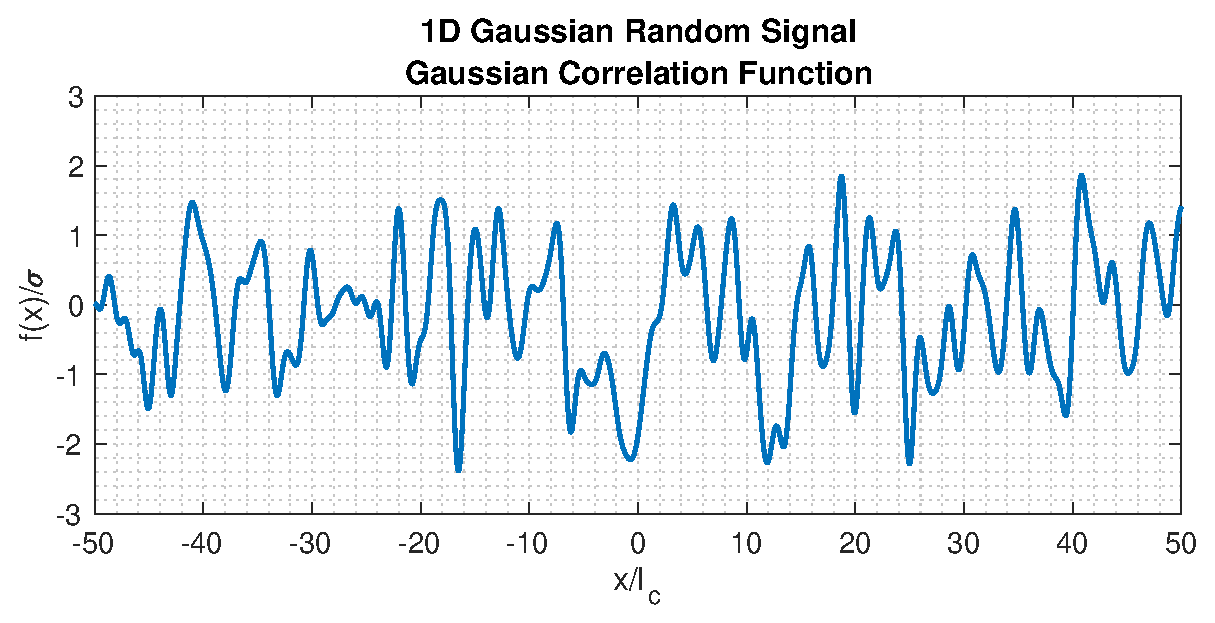
\includegraphics[width=4in]{RandomObjects/Figures/gaussiansurf1} } \\
    \subfigure{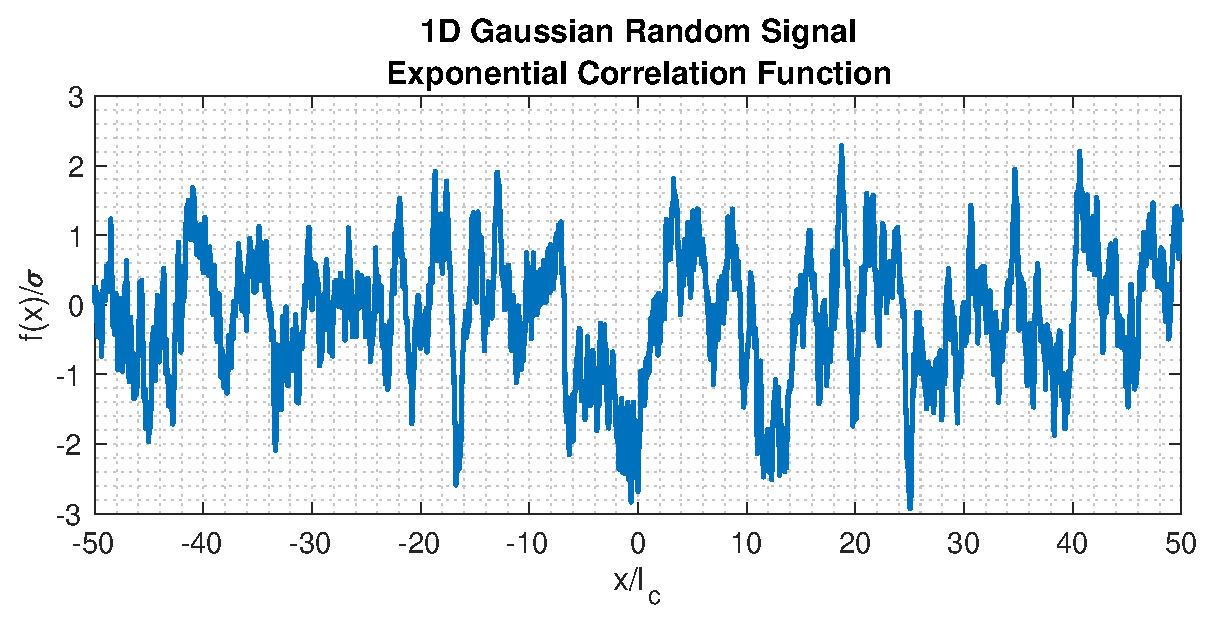
\includegraphics[width=4in]{RandomObjects/Figures/gaussiansurf2} }
    \caption{1D Gaussian random signals with Gaussian and exponential correlation functions generated from the same random seed. The vertical and horizontal axes are normalized by the RMS and correlation length, respectively. Note, signals with an exponential correlation function always have a discontinuous derivative no matter how finely they are sampled.}
\end{figure}



The spectrum of a 1D rough surface with physical length $L_x$ is given by
\begin{equation}
F(k_x) = \gamma(k_x)\sqrt{\delta k_x W(k_x)}
\end{equation}

\noindent where $\delta k_x = 2 \pi/ L_x$ and $\gamma(k_x)$ is an independent draw from the complex standard normal distribution for each spatial frequency $k_x$.  It is $\gamma$ that imparts randomness to each realization of the PSD.  The complex standard normal is defined:
\begin{equation}
\gamma = \dfrac{1}{\sqrt{2}}\left( \mathcal{N}(0,1) + i \mathcal{N}(0,1)\right)
\end{equation}

\noindent where $\mathcal{N}(0,1)$ is the standard normal distribution with zero mean and unit variance. $\gamma$ is normalized so that its variance is one.  Finally, the surface is realized with an inverse Fourier transform:
\begin{equation}
f(x) = \mathcal{F}_{k_x}^{-1}\left[F(k_x)\right]
\end{equation}

Another important quantity is the variance of the difference of surface heights as a function of lag. This is called the Allan variance. The square root of this quantity is the Allan deviation or RMS deviation. The deviation is zero at zero lag and grows following the correlation function until points separated by more than the correlation length become uncorrelated and the variance is equal to two times the variance of the underlying process. The variance at lag $\Delta x$ is 
\eq{v^2(\Delta x) = 2 \sigma^2 \left(1 - C(\Delta x)\right)}

Then the RMS deviation at lag $\Delta x$ is 
\eq{v(\Delta x) = \sqrt{2} \sigma \sqrt{\left(1 - C(\Delta x)\right)}}



%
% \begin{figure}[H] 
%   \centering
%   \subfigure{\includegraphics[width=3in]{RandomObjects/Figures/gaussiansurf} }
%    \subfigure{\includegraphics[width=3in]{RandomObjects/Figures/gaussiancorr} }\\
%     \subfigure{\includegraphics[width=3in]{RandomObjects/Figures/gaussiandev} }
%    \caption{1D Gaussian random signals with Gaussian and exponentially correlation functions. Note, a signal with exponential correlation function always has discontinuous derivative no matter how fine the sampling.}
%\end{figure}
%



The routine \texttt{rough1} generates a real-valued zero-mean 1D Gaussian random signal. The inputs are the number of points $N_x$, length of the signal $L_x$, RMS height $\sigma$, correlation length $l_c$. Use string switch \texttt{norm} or \texttt{exp} for Gaussian or exponential correlation functions. When the correlation length is less than the sample size, and therefore the signal is not properly sampled, the routine returns independent draws from a Gaussian distribution at each point with the given RMS. When generating a real valued signal from its spectrum, we usually make the spectrum conjugate symmetric before taking the IFFT. Instead, it is easier to seed the PSD with samples from an unnormalized non-conjugate complex standard normal distribution and then take the real part of the IFFT.  Matlab's \texttt{ifft} divides by the number of samples in each dimension, so to keep the transform independent of domain size, this factor has to be put back. The 1D PSDs are coded inline, but can be plotted separately by the routines \texttt{psdnorm} and \texttt{psdexp}.  


  {\footnotesize
\VerbatimInput{\code/RandomObjects/rough1.m}
}

%
%{\footnotesize
%\VerbatimInput{\code/RandomObjects/psdnorm.m}
%}
%
%{\footnotesize
%\VerbatimInput{\code/RandomObjects/psdexp.m}
%}

%
%
% \begin{figure}[h] 
%   \centering
%   \includegraphics[width=4in]{RandomObjects/Figures/rough1} 
%   \caption{1D Gaussian and exponentially correlated rough surfaces with 0.1 RMS and 3 m correlation length generated with the same random seed.  Note that the exponential correlation function yields a function with discontinuous derivative.}
%\end{figure}
%
% \begin{figure}[h] 
%   \centering
%   \includegraphics[width=4in]{RandomObjects/Figures/rough1_corr} 
%   \caption{1D Gaussian and exponentially computed correlation functions. }
%\end{figure}



\section{2D Random Surfaces}

A 2D random rough surface is like a beach or patch of dirt, which is a height map of two variables.  2D rough surfaces are created like 1D random signals, except that the PSDs acquire an extra dimension and scaling factors. In addition, anisotropic correlations are now possible. Gaussian and exponential correlation functions are given by
\ea{C(\Delta x, \Delta y) &=& \exp\left(-\dfrac{\Delta x^2}{l_{cx}^2}-\dfrac{\Delta y^2}{l_{cy}^2}\right) \\
C(\Delta x, \Delta y) &=& \exp\left(-\sqrt{\dfrac{\Delta x^2}{l_{cx}^2} + \dfrac{\Delta y^2}{l_{cy}^2} }  \right)}

The corresponding power spectral densities are 
\ea{W(k_x,k_y) &=& \dfrac{\sigma^2 l_{cx} l_{cy}}{4\pi}\exp\left(-\dfrac{k_x^2 l_{cx}^2}{4}-\dfrac{k_y^2 l_{cy}^2}{4}\right) \\
W(k_x,k_y) &=& \dfrac{\sigma^2 l_{cx}l_{cy}}{2\pi\left(1+k_x^2l_{cx}^2+k_y^2l_{cy}^2\right)^{3/2}}}

The 2D frequency spectrum is given by
\begin{equation}
F(\bb{k}) = \gamma(\bb{k})\sqrt{\delta k_x \delta k_y W(\bb{k})} 
\end{equation}
\begin{equation}
\begin{array}{ccc}
\delta k_x = \dfrac{2\pi}{L_x} & \delta k_y = \dfrac{2\pi}{L_y} & k = \sqrt{k_x^2 + k_y^2}
\end{array}
\end{equation}

Here, $\gamma(\bb{k})$ is the complex standard normal distribution evaluated independently at each $\bb{k}$.  

\begin{figure}[H] 
   \centering
 \subfigure{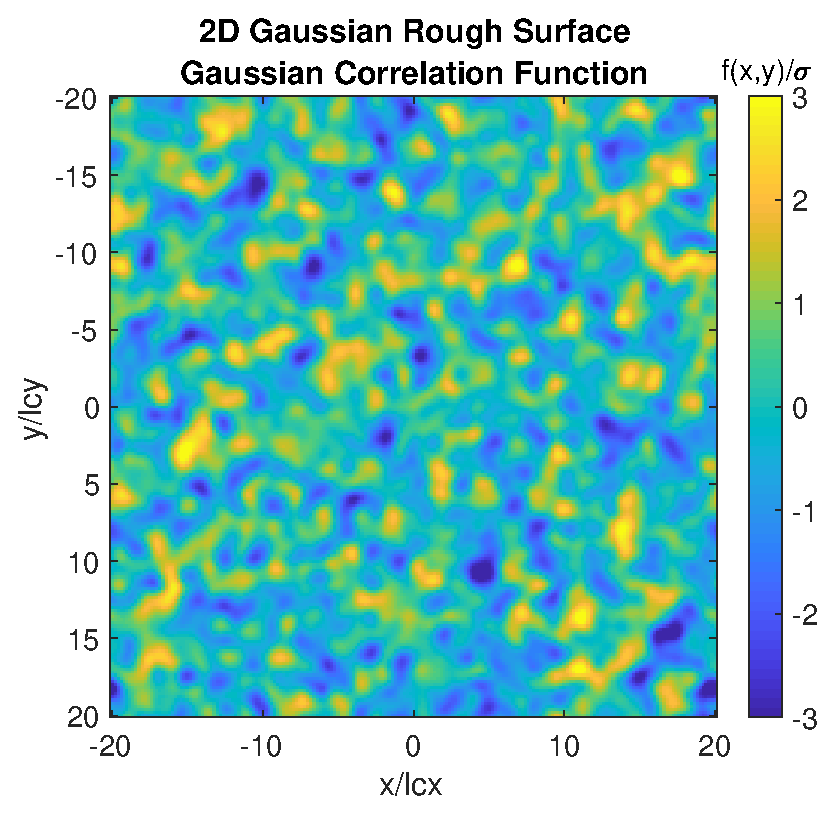
\includegraphics[width=2.5in]{RandomObjects/Figures/rough2norm}}
  \subfigure{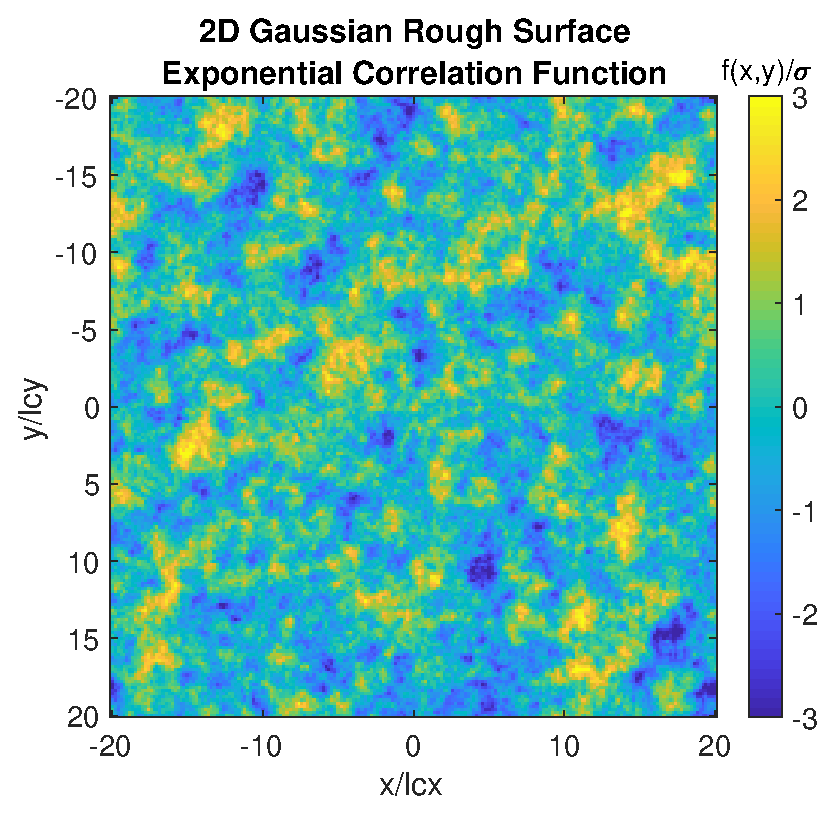
\includegraphics[width=2.5in]{RandomObjects/Figures/rough2exp}}
   \caption{2D Gaussian and exponentially correlated rough surfaces generated with the same random seed. The surface height is normalized by the RMS, and the axes are normalized by the correlation length.}
\end{figure}


The routine \texttt{rough2} generates a real-valued zero-mean 2D Gaussian random surface. The inputs are the number of points $N_x$, $N_y$ in each dimension, side lengths of the domain $L_x$, $L_y$, RMS height $\sigma$, and correlation lengths in each dimension $l_{cx}$, $l_{cy}$. It returns the surface in \texttt{meshgrid} format. Use string switch \texttt{norm} or \texttt{exp} for Gaussian or exponential correlation functions. As in the 1D case, we can avoid having to make the spectrum conjugate symmetric by drawing from the unnormalized non-conjugate complex standard normal and then simply taking the real part of the 2D IFFT. If the correlation lengths in both dimensions are less than their respective sample sizes, the surface heights are independent draws from a Gaussian distribution. If the correlation length of one dimension is less than its sample size, then we treat the other dimension as a collection of independent 1D rough surfaces. These provisions help maintain the correct RMS height when the PSD is poorly sampled. 

{\scriptsize %\footnotesize
\VerbatimInput{\code/RandomObjects/rough2.m}
}

\clearpage


\section{3D Random Volumes}

A 3D rough volume represents random fluctuations in space, such as random dielectric material or density variations. The Gaussian and exponential correlation functions are
\ea{C(\Delta x, \Delta y, \Delta z) &=& \exp\left(-\dfrac{\Delta x^2}{l_{cx}^2}-\dfrac{\Delta y^2}{l_{cy}^2} - \dfrac{\Delta z^2}{l_{cz}^2 }\right) \\
C(\Delta x, \Delta y, \Delta z) &=& \exp\left(-\sqrt{\dfrac{\Delta x^2}{l_{cx}^2} + \dfrac{\Delta y^2}{l_{cy}^2} + \dfrac{\Delta z^2}{l_{cz}^2} }  \right)}

The corresponding power spectral densities are
\ea{W(k_x,k_y,k_z) &=& \dfrac{\sigma^2 l_{cx} l_{cy} l_{cz}}{8\pi^{3/2}}\exp\left(-\dfrac{k_x^2 l_{cx}^2}{4}-\dfrac{k_y^2 l_{cy}^2}{4}-\dfrac{k_z^2 l_{cz}^2}{4}\right) \\
W(k_x,k_y,k_z) &=& \dfrac{\sigma^2 l_{cx}l_{cy}l_{cz}}{3\pi\left(1+k_x^2l_{cx}^2+k_y^2l_{cy}^2+k_z^2l_{cz}^2\right)^{2}} }

The spectrum is then 
\begin{equation}
F(\bb{k}) = \gamma(\bb{k})\sqrt{\delta k_x \delta k_y \delta k_z W(\bb{k})} 
\end{equation}
\begin{equation}
\begin{array}{cccc}
\delta k_x = \dfrac{2\pi}{L_x} & \delta k_y = \dfrac{2\pi}{L_y} & \delta k_z = \dfrac{2\pi}{L_z} & k = \sqrt{k_x^2 + k_y^2 + k_z^2}
\end{array}
\end{equation}


 \begin{figure}[H] 
    \subfigure{
   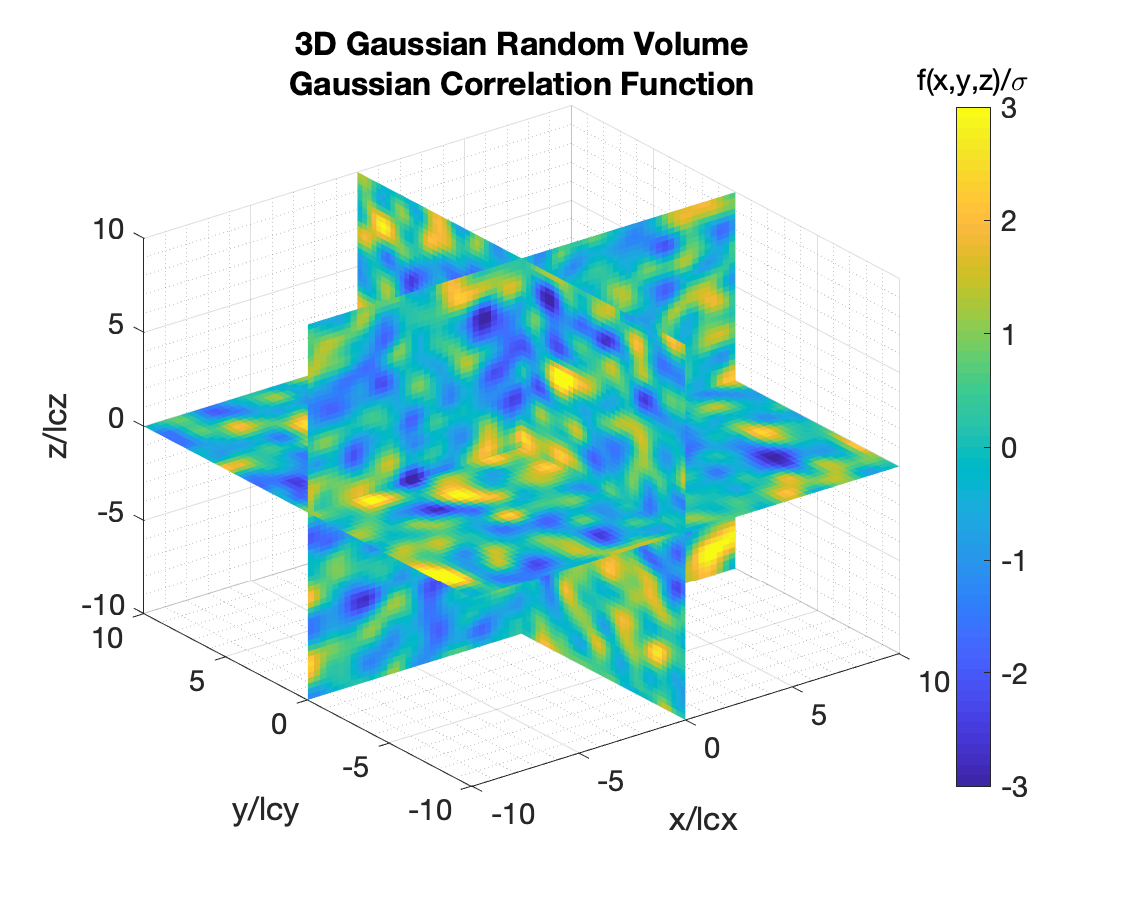
\includegraphics[width=3in]{RandomObjects/Figures/gauss3Dnorm} } 
   \subfigure{
    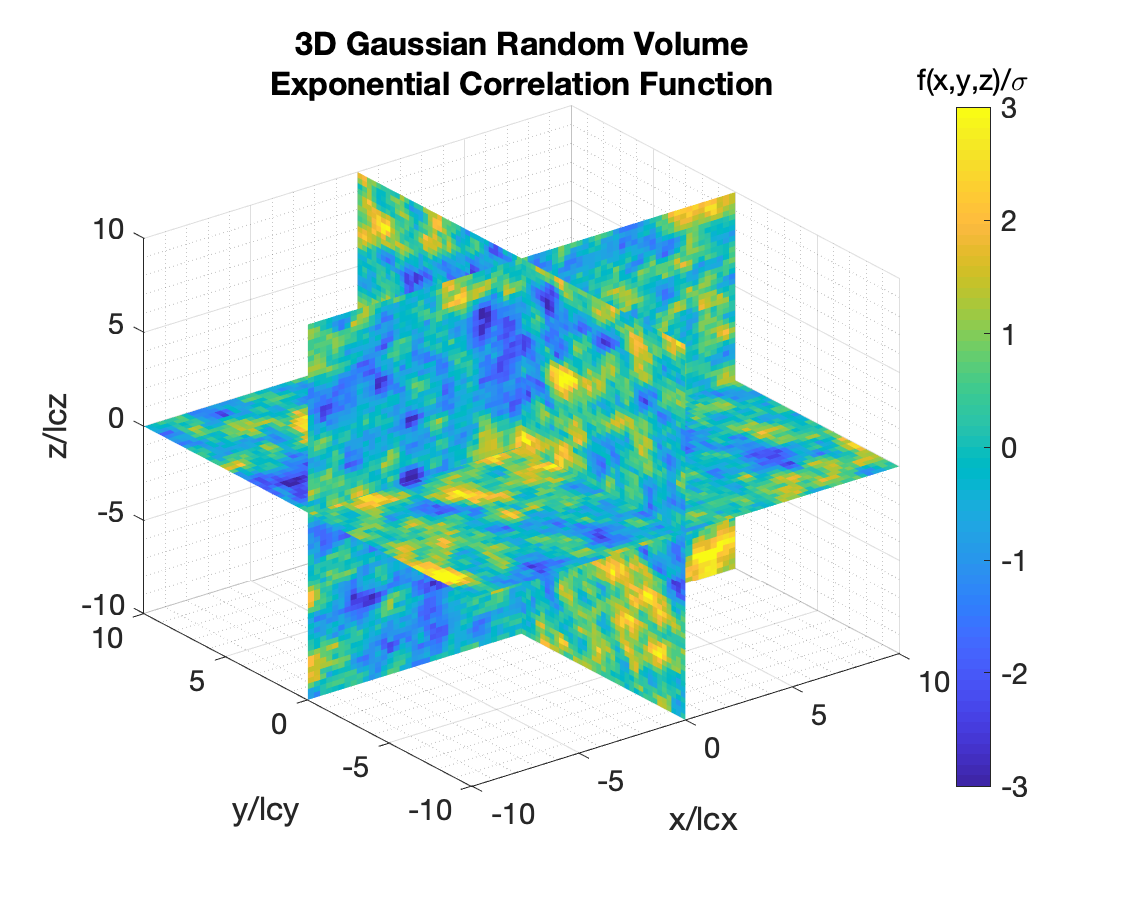
\includegraphics[width=3in]{RandomObjects/Figures/gauss3Dexp} } 
   \caption{3D Gaussian and exponential correlated random volumes generated with the same seed. The function value is normalized by the RMS, and the axes are normalized by the correlation length.}
\end{figure}



The routine \texttt{rough3} generates a real-valued zero-mean 3D Gaussian random volume. The inputs are the number of points $N_x$, $N_y$, $N_z$ in each dimension, side lengths of the domain $L_x$, $L_y$, $L_z$, RMS fluctuation $\sigma$, and correlation lengths in each dimension $l_{cx}$, $l_{cy}$, $l_{cz}$.  It returns the volume in \texttt{meshgrid} format. Use string switch \texttt{norm} or \texttt{exp} for Gaussian or exponential correlation functions. If the correlation lengths in all dimensions are less than their respective sample sizes, the values are independent draws from a Gaussian distribution. If correlation lengths in two dimensions are less than their sample sizes, the third dimension is composed of independent 1D random signals. If the correlation length of one dimension is less than its sample size, the other two dimensions are independent 2D random signals. 

\clearpage
{\footnotesize
\VerbatimInput{\code/RandomObjects/rough3.m}
}


\clearpage
\newpage

\section{1D Fractal Signals}

Fractal signals are a class of Gaussian random process that are self-similar at increasing length scales. In short, the RMS grows as the profile length grows. Equivalently, these signals describe fractional Brownian motion, of which traditional Brownian motion is a subset. For in-depth explanations of fractal surfaces, theory, and relation to natural surfaces, see \cite{shepard1995self,shepard1999radar}. For details on computing these signals quickly, see \cite{kroese2015spatial}.  

The statistics of 1D fractal signals are described by either an RMS height (or variance) over all points which depends on total length of the profile, or the RMS deviation (or Allan variance), that depends on the relative positions, or lag, between pairs of points. For a 1D profile with height $z(x)$, the variance of the heights is computed as 
\eq{\sigma^2 = \left< (z - \bar{z})^2 \right> }

and the Allan variance is computed as
\eq{v^2 = \left< (z(x) - z(x + \Delta x))^2 \right>}

\noindent where $ \Delta x$ is the lag and $\left< \right>$ is the ensemble average.  For natural fractal surfaces, these quantities can be described by a power law such that the RMS height over the entire profile length, $x$, is
\eq{\sigma(x) = \sigma_o \left( \dfrac{x}{x_o}\right)^H \label{rmsh} }

\noindent where $\sigma_o$ is the RMS height at length scale $x_o$, and $H$ is the Hurst exponent, which takes values $0 \le H \le 1$. Alternatively, the surface can be described by a power law such that the RMS deviation (Allan deviation, or just deviation) at lag $\Delta x$ is given by
\eq{v(\Delta x) = v_o \left( \dfrac{\Delta x}{\Delta x_o}\right)^H \label{rmsv}}

\noindent where $v_o$ is the RMS deviation at lag $\Delta x_o$, and $\Delta x$ is the lag at which we evaluate the deviation. The Hurst exponent controls the growth of the surface over distance, while the other parameters simply scale the result. The statistics of both the surface height and variation are Gaussian. When $H=1/2$ the process becomes standard 1D Brownian motion.

\begin{figure}[H] 
   \centering
   \subfigure{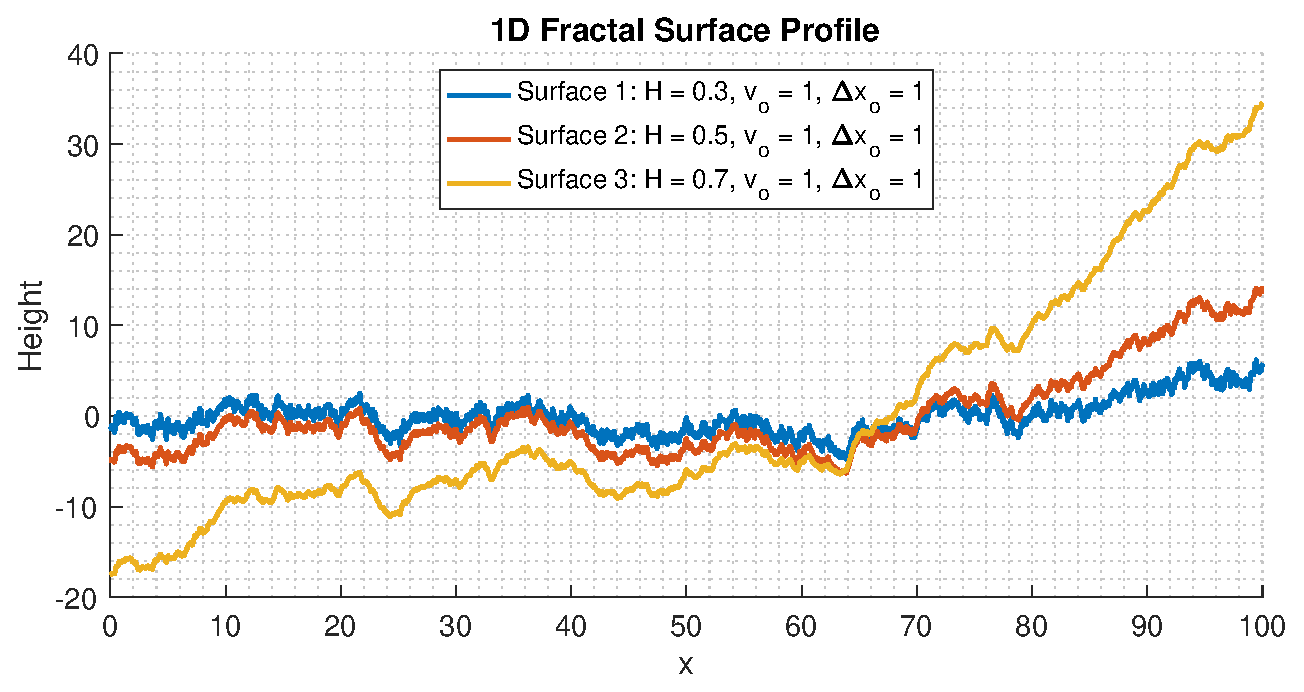
\includegraphics[width=3.2in]{RandomObjects/Figures/fracsurf}} 
   \subfigure{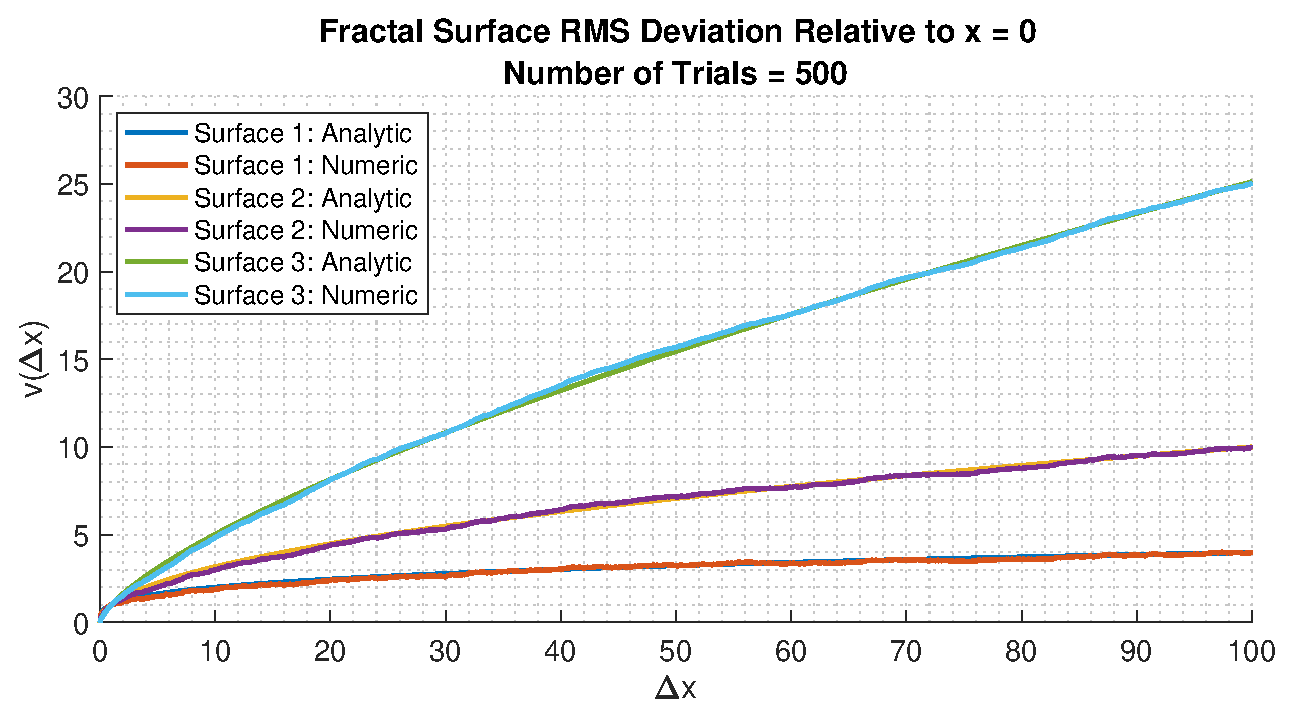
\includegraphics[width=3.2in]{RandomObjects/Figures/fracdiffvrms}}
   \caption{Top: 1D fractal profiles generated from the same seed.  Bottom: RMS deviation relative to $x = 0$, $v(\Delta x)$, analytic and numeric computed over 500 trials. This shows how the deviation of the fractal surface continues to grow with length scale. }
\end{figure}


From \cite{shepard1995self}, the RMS slope is defined
\eq{s_{rms} = \sqrt{\left< \left(\dfrac{\Delta z}{\Delta x}\right)^2 \right > }}
The RMS of $\Delta z$ is just \eqref{rmsv}, therefore, the RMS slope is
\eq{s_{rms} = \dfrac{v(\Delta x)}{\Delta x} = v_o \left( \dfrac{\Delta x}{\Delta x_o}\right)^{H-1} \label{rmsslope} }


%From \cite{kroese2015spatial}, the covariance of the random variables of two heights, $X_1$ and $X_2$, at two points $x_1$ and $x_2$, is given by 
%
%\eq{\textrm{Cov}[X_1,X_2] = \dfrac{1}{2}\left(\vert x_1 \vert^{2H} + \vert x_2 \vert^{2H}  - \vert x_1 - x_2 \vert^{2H}\right)}

%For example, the PDF of surface variation $\bar{z} = z - z(0)$ as a function of lag is 
%\eq{f_z(\bar{z} \vert \Delta x) = \dfrac{1}{\sqrt{2\pi} v(\Delta x)}\exp\left(-\dfrac{1}{2}\dfrac{\bar{z}^2}{ v^2(\Delta x)}\right)}


The routine \texttt{fractal1} generates a zero-mean 1D fractal signal based on the routine in \cite{kroese2015spatial}, to which we have added options for normalization by RMS height or RMS deviation. It takes as input the pair ($\sigma_o$, $x_o$) or ($v_o$, $\Delta x_o$), the Hurst exponent $H$, the number of sample points, and the length of the profile. Use string switch \texttt{'rms'} or \texttt{'dev'} for normalization by RMS height or RMS deviation. The signal generated by \cite{kroese2015spatial} was found to scale perfectly for RMS deviation, \eqref{rmsv}. For RMS height, the signal is simply rescaled by \eqref{rmsh}. 

{\footnotesize
\VerbatimInput{\code/RandomObjects/fractal1.m}
}



\clearpage
\newpage

\section{Bicontinuous Random Media}

Bicontinuous random media are used to model 2-species material with different levels of connectivity. For example, these have been used to model the distribution of ice/void volumes of settled snow that have different amounts of melting and compaction, \cite{ding2010electromagnetic,xu2012electromagnetic,chang2016microwave,tan2016uniaxial}. Bicontinuous random media partition the volume into binary regions by cutting a fluctuating 3D field at a prescribed level and then assigning the material based on whether the value of the field is above or below the level cut at a given point. The field has Gaussian statistics, therefore the cutting level corresponds to the volume fraction of the binary regions. We outline the components of the model given in \cite{ding2010electromagnetic,xu2012electromagnetic} for isotropic bicontinuous random media, while an anisotropic model can be found in \cite{tan2016uniaxial}.

\paragraph{Distribution} The 3D fluctuating field is a sum of random plane waves 
\eq{S(\br) = \dfrac{1}{\sqrt{N}} \sum_{n=1}^N \cos\left(\bb{k}_n \cdot \br + \phi_{n} \right) \label{flutuatingfieldbicont}}

\noindent where $S(\br)$ is the fluctuating field, $N$ is the number of wave vector directions, $\bb{k}_n$ is the wave vector, and $\phi_n$ is a random phase. The wave vector directions, $\hat{k}_n$, are distributed uniformly random over the sphere. The wave vector magnitudes, $k_n$, are drawn from a gamma distribution. The phase is drawn from a uniform random variable between 0 and $2\pi$.  The gamma distribution for the wave vector amplitudes is given by, \cite{ding2010electromagnetic},
\eq{p(k) = \dfrac{1}{\Gamma(b+1)}\dfrac{(b+1)^{b+1}}{\left< k\right>} \left(\dfrac{k}{\left< k\right>}\right)^b e^{-(b+1) \frac{k}{\left< k\right>}} \label{gammasnow}}

\noindent where $\Gamma$ is the gamma function, $\left< k\right>$ is the mean wavenumber and $b$ is a constant. Physically, $\left< k\right>$ corresponds to the reciprocal of the average length scale of heterogeneity (average snow grain size), while $b$ corresponds to the width of the distribution (spread of snow grain size) \cite{xu2012electromagnetic}. Despite its appearance, \eqref{gammasnow} is equivalent to the common form of the gamma distribution that has shape parameter $b+1$ and scale parameter $\left< k\right>/(b+1)$. These parameters are needed to draw samples from built-in routines. The mean of the distribution is $\left< k\right>$ and the standard deviation is $\sigma = \left< k\right>/\sqrt{b+1}$.

An indictor function is used to assign the binary classification to each point in the field based on a level cut. The indicator function is 
\eq{\Theta(S(\br)) = \begin{cases} 1, & S(\br) > \alpha \\
0, & S(\br) \le \alpha \end{cases}}

\noindent where $\Theta(\br)$ is the indicator function and $\alpha$ is the cutting level.  The statistics of the field are zero-mean Gaussian with variance 1/2. Because of this, the fractional volume, $f_v$, of the 1 indicator is related to the cutting level as 
\eq{f_v = \dfrac{1}{2}\left(1 - \textrm{erf}(\alpha)\right)}

\noindent where $\textrm{erf}$ is the error function.  The cutting level is given in terms of the fractional volume as 
\eq{\alpha = \textrm{erf}^{-1}\left(1 - 2f_v\right)}

\noindent where $\textrm{erf}^{-1}$ is the inverse error function.

The construction of \eqref{flutuatingfieldbicont} as a sum over spatial plane waves has several interesting consequences. The direct sum, together with the fact that $N$ needs to be large, makes the computation slow over a large number of points. In \cite{ding2010electromagnetic} a value of $N = 10^4$ is used, though we have found that $N=10^3$ suffices. Also, because this does not use a PSD, FFT methods cannot be used to accelerate the computation. However, precisely because \eqref{flutuatingfieldbicont} is spatially sampled and not based on a PSD or FFT, the 3D field and indicator function can be computed at arbitrary points, for example, along 1D lines, 2D sheets, or 3D volumes. This allows large volumes to be computed in pieces by using the same random seed.

\newpage 
\paragraph{Correlation Function}

The spatial correlation function of $\Theta(\br)$ is radially symmetric and given by, \cite{ding2010electromagnetic}, 
\eq{\Gamma_{\alpha}(r) = f_v^2 + C_{\alpha}(r)}

\noindent where 
\ea{C_{\alpha}(r) &=& \sum_{m=1}^{\infty} C_m(\alpha) \left[ C_s(r)\right]^m \\
C_m(\alpha) &=& \dfrac{e^{-2\alpha^2} \left[H_{m-1}(\alpha)\right]^2}{\pi m! 2^m} \\
C_s(r) &=& \dfrac{\sinc(b\varphi)}{\sinc(\varphi)} \cos^{b+1}(\varphi) \\
\varphi &=& \textrm{tan}^{-1}\left(\dfrac{\left< k\right> r}{b+1} \right)}

\noindent where $C_{\alpha}(r) = \Gamma_{\alpha}(r) - f_v^2$ and $C_s(r)$ is the autocovariance of $S(\br)$. The coefficients, $C_m(\alpha)$, are given in terms of the Hermite polynomials, $H_m(x)$. In addition, $\sinc(x) = \sin(x)/x$.  Finally, $\Gamma_{\alpha}(0) = f_v$, $\Gamma_{\alpha}(\infty) = f_v^2$, $C_s(0) = 1$, and $C_s(\infty) = 0$. 

%The coefficients $C_m(\alpha)$ can be computed using the log transform, $C_m(\alpha) = e^{\ln C_m(\alpha)}$, and the following recursion relation
%\ea{\ln C_{m+1}(\alpha) &=& \ln C_m(\alpha) + 2(\ln H_{m} - \ln H_{m-1}) - \ln (m+1)  - \ln 2 \\
%\ln C_{1}(\alpha) &=&  -2\alpha^2 - \ln\pi  - \ln 2 }
%
%\ea{\ln C_m(\alpha) &=& -2\alpha^2 + 2\ln H_{m-1} - \ln\pi - \ln m! - m \ln 2 \\
%\ &=& -2\alpha^2 + 2\ln H_{m-1} - \ln\pi - \sum_{k=1}^m \ln k - m \ln 2}
%
%Evaluating at $m+1$
%\ea{\ln C_{m+1}(\alpha) &=& -2\alpha^2 + 2\ln H_{m} - \ln\pi - \sum_{k=1}^{m+1} \ln k- (m+1) \ln 2 \\
%&=& -2\alpha^2 + 2\ln H_{m}  + 2\ln H_{m-1}  - 2\ln H_{m-1} - \ln\pi - \sum_{k=1}^m \ln k - \ln (m+1) - m \ln 2 - \ln 2 \\
%&=& \ln C_m(\alpha) + 2(\ln H_{m} - \ln H_{m-1}) - \ln (m+1)  - \ln 2}
%
%Finally, the Hermite polynomials can be computed inline with the recursion 
%\eq{H_{m+1}(x) = 2xH_m(x) - 2mH_{m-1}(x)}
%
%and initial conditions $H_0(x) = 1$ and $H_1(x) = 2x$. 

 \begin{figure}[H] 
 \centering
   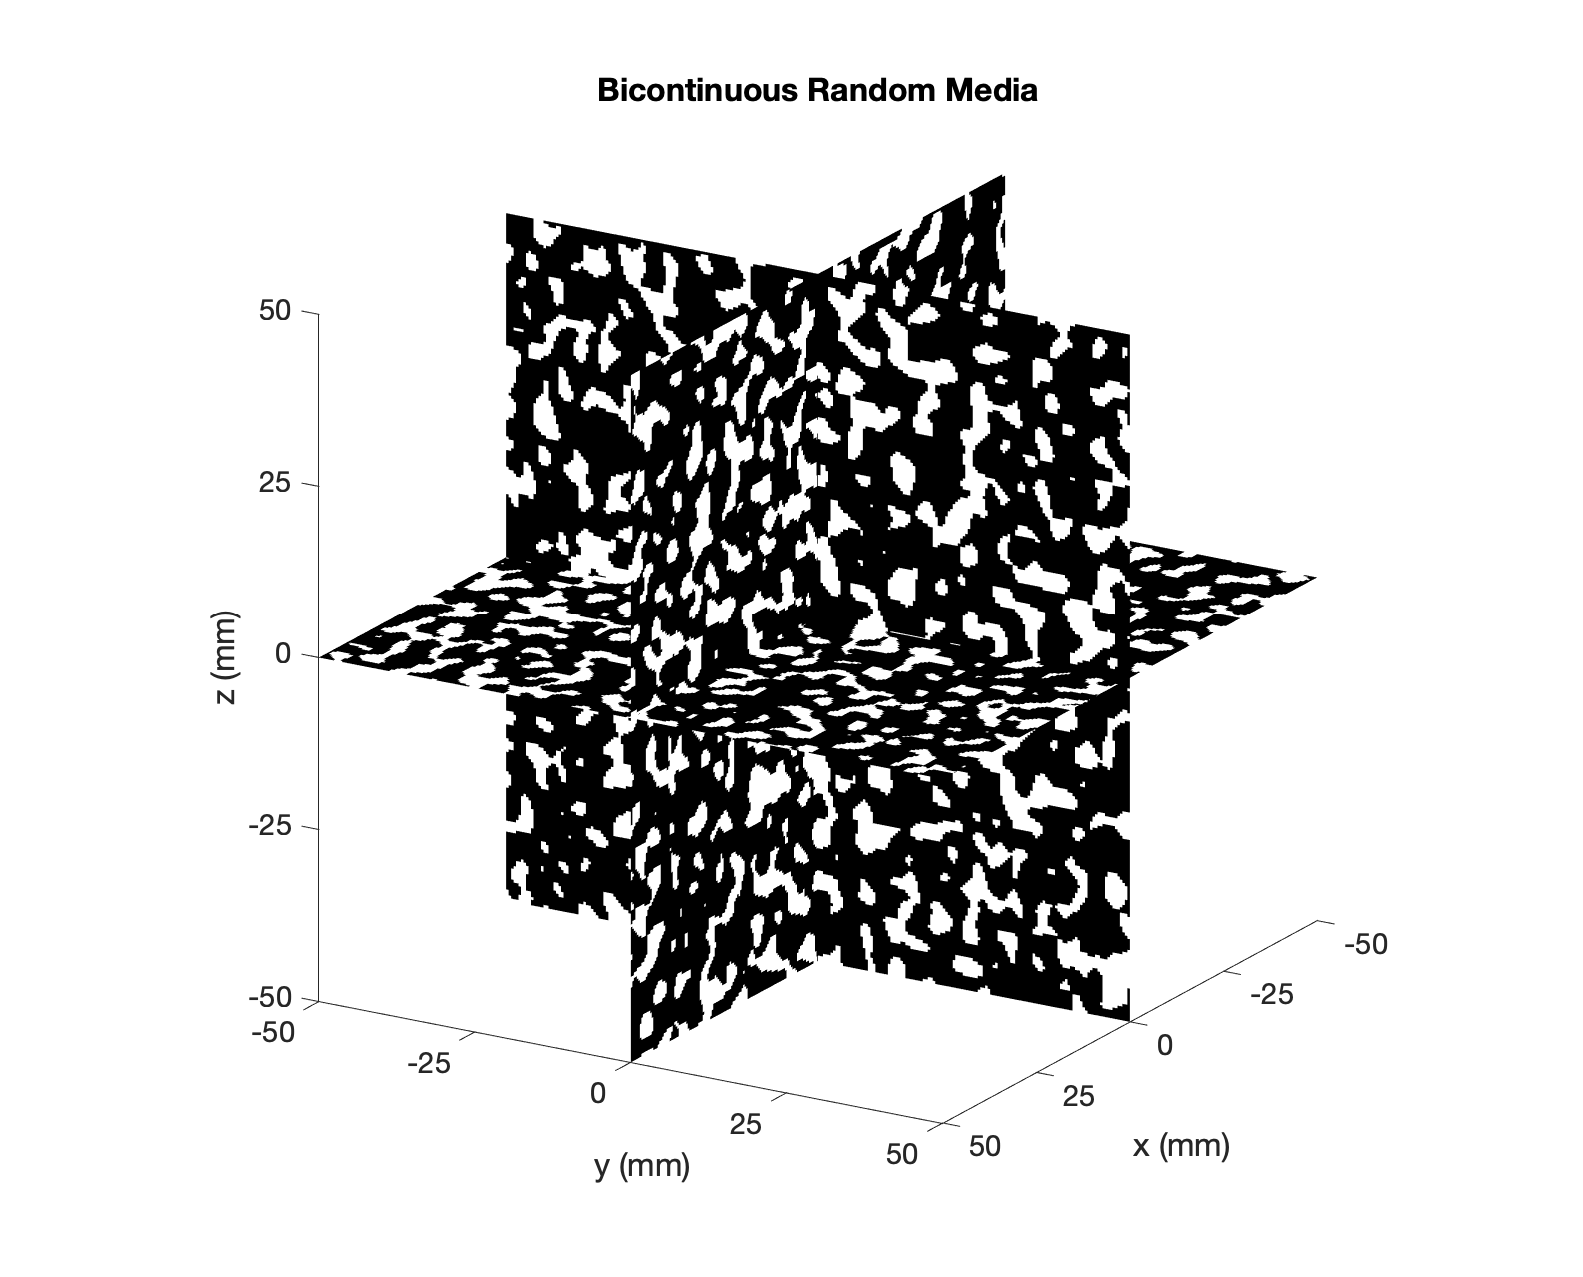
\includegraphics[width=4.5in]{RandomObjects/Figures/bicont} 
      \caption{Bicontinuous random media for $l_{ave} = 2\pi/\left< k\right> = 5$ mm, $b= 10$, and $f_v$ = 0.3. The 2D slices of the same field are computed separately by running the routine again with the same random seed. }
\end{figure}


\paragraph{Routine}

The routine \texttt{bicont} returns the bicontinuous indicator function, $\Theta(\br)$. It takes as input the arrays of the Cartesian coordinates $\br = (x,y,z)$, which can be any size, the mean length scale of the heterogeneity, $l_{ave}$, spreading parameter, $b$, and fractional volume, $f_v$. The mean length scale is converted to mean wavenumber as $\left<k\right> = 2\pi/l_{ave}$. $l_{ave}$ needs to have the same units as the coordinates. The number of plane waves, $N$, is optional and defaults to $N=10^3$. Random plane directions are computed with our routine \texttt{randsphere}. This relies on Matlab routines \texttt{gamrnd} and \texttt{erfinv} which require certain toolboxes. The fluctuating field, $S(\br)$, is an optional output. 

%Finally, the routine \texttt{bicontcorr} returns the three correlation functions, $\Gamma_{\alpha}(r)$, $C_{\alpha}(r)$, and $C_s(r)$, computed with the recursion method above using inputs of radial distance, $r$, and distribution parameters $l_{ave}$, $b$, and $f_v$.

\clearpage
{\footnotesize
\VerbatimInput{\code/RandomObjects/bicont.m}
}

%\newpage

%\section{2D Fractal Surfaces}


\newpage

\section{Ocean Waves}

Ocean wave scenes are generated as a 2D rough surface. Ocean waves have a nonlinear dispersion relation, so some care is needed when deriving the power spectral density. Models for temporal evolution also come in linear and nonlinear flavors, but all use the same underlying PSD. Note, only one realization of the ocean spectrum is needed in order to evolve the surface in time.
  
\begin{figure}[h] 
   \centering
   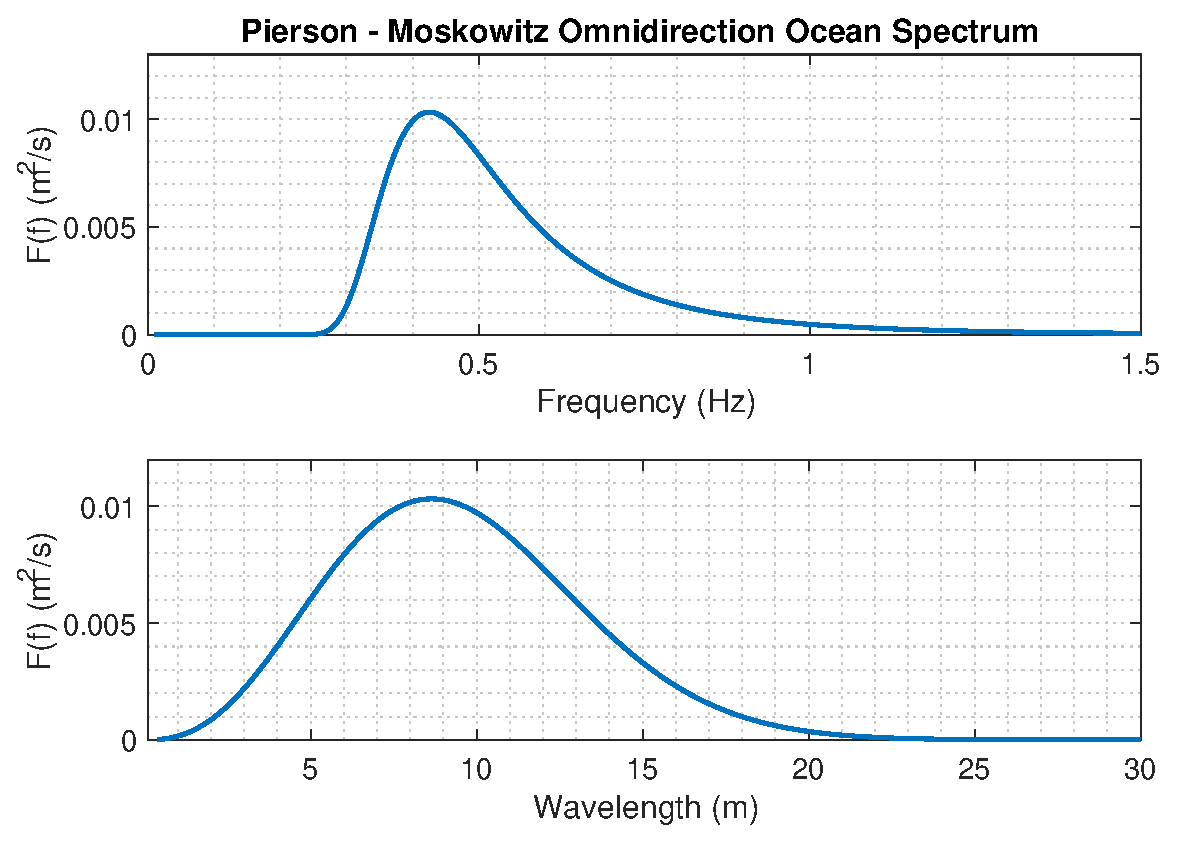
\includegraphics[width=4in]{RandomObjects/Figures/pmspectrum} 
   \caption{Pierson-Moskowitz spectrum for $U_{10} = 3$ m/s}
\end{figure}

The classic Pierson-Moskowitz (PM) omnidirectional wave spectrum for fully developed ocean waves is 
\begin{equation}
F(f) = \dfrac{\alpha g^2}{\left(2\pi\right)^4 f^{5}} \textrm{exp}\left[-(5/4)\left(\dfrac{f_p}{f}\right)^4\right]
\end{equation}

\noindent where $\alpha = 0.0081$ is the Phillips constant, $g = 9.81$ m/s$^2$ is gravitational acceleration, $f$ is the spectral frequency, and $f_p$ is the peak frequency, both frequencies have units of Hz \cite{alves2003revisiting}.  This is an omnidirectional spectrum; angular variation will be added later to account for wind direction. The peak frequency is given empirically as 
\begin{equation}
f_p = 0.13 \dfrac{g}{U_{10}}
\end{equation}

\noindent where $U_{10}$ is the wind speed 10 meters above the mean surface level.  The variance of the wave height is given by the integral over the density function 
\eq{\sigma^2 = \int_0^{\infty} F(f) df  = \dfrac{\alpha g^2}{\left(2\pi\right)^4 5 f_p^4 }}

The RMS wave height is then 
\eq{\sigma = \dfrac{\sqrt{\alpha} g}{\left(2\pi\right)^2 \sqrt{5} f_p^2 } \label{oceanrms} }

The dispersion relation for ocean waves is $\omega^2  = g k$ from which it follows that the phase velocity, group velocity, and wavelength are
\begin{eqnarray}
v_p &=& \dfrac{\omega}{k} = \sqrt{\dfrac{g}{k}} \\
v_g &=& \dfrac{d\omega}{dk} = \dfrac{g}{2\omega} \\
\lambda & = & \dfrac{g}{2 \pi f^2}
\end{eqnarray}

To create wave scenes, the omnidirectional spectrum given in frequency needs to be converted to 2D $k$-space.  This requires a change of variables.  If one desires the 1D ocean spectra in $k$-space, the change of variables via the Jacobian is explained in \cite{tolman2009user}.  How to convert to the 2D omnidirectional spectra is explained in \cite{plant2009ocean} and repeated here.  The total wave height variance integrated over all angles must not depend on the independent variable, $f$ or $k$.  This condition is met when 
\begin{equation}
\int F(k) k dk = \int F(f) df
\end{equation}

\noindent which yields the change of variables
\begin{equation}
F(k) = F(f) \dfrac{df}{k dk} = F(f) \dfrac{d\omega}{2\pi k dk} = F(f) \dfrac{v_g}{2\pi k}
\end{equation}

\noindent where $F(k)$ is the 2D omnidirectional spectrum.  Next, the 2D PSD is the product of the omnidirectional spectrum and an angle dependent spreading function \cite{soriano2006doppler}:
\begin{equation}
W(\bb{k}) = F(k)\phi(\theta)
\end{equation}

\noindent where $\bb{k}$ is the 2D wavenumber and $(k,\theta)$ are its polar coordinates.  The spreading function can take a few forms, most are some power of $\cos(\theta)$, given in \cite{soriano2006doppler} as
\begin{equation}
\phi(\theta) = \dfrac{1}{N} \biggl \vert \cos^5\left(\dfrac{\theta-\theta_{\textrm{v}}+\pi}{2}\right) \biggr \vert
\end{equation}

\noindent where $\theta_{\textrm{v}}$ is the direction from which the wind is blowing (meteorological convention).  The normalization is $N = \int_{-\pi}^{\pi} \vert \cos^5(\theta/2)\vert d\theta = 32/15$.  More general spreading functions are given in \cite{hasselmann1980directional,niedzwecki1991comparative}.  A factor of $\pi$ has been added to the argument to give the spectrum the correct orientation relative to our definition of the wind direction, the $k$-vectors, and FFT convention.  

\begin{figure}[htbp] 
   \centering
   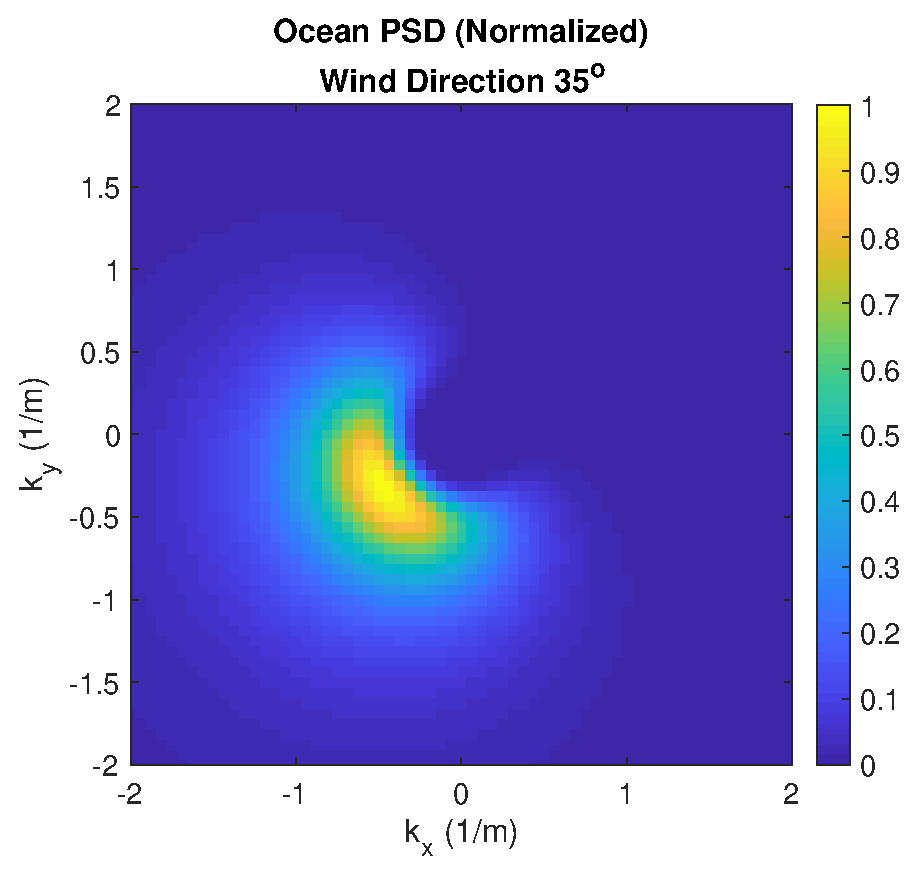
\includegraphics[width=2.5in]{RandomObjects/Figures/oceanPSD} 
   \caption{2D ocean PSD (normalized) for $U_{10} = 3$ m/s, and $\theta_{\textrm{v}} = 35^o$. Most waves travel downwind, some have an upwind component, none travel directly upwind.}
\end{figure}

From \cite{soriano2006doppler, niedzwecki1991comparative}, the complex amplitude of the wave heights at time $t$ is given by
\begin{equation}
A(\bb{k},t) = \gamma(\bb{k})\sqrt{\delta k_x \delta k_yW(\bb{k})} e^{-i\omega t}
\end{equation}

\noindent where $\gamma(\bb{k})$ is the complex standard Gaussian distribution.  $\omega$ is replaced with the dispersion relation, $\sqrt{gk}$, giving a spectrum in terms of $k$ and $t$. The effect of the nonlinear dispersion relation is that different parts of the spatial spectrum oscillate at different rates in time.  The steps are $\delta k_x = 2\pi/L_x$ and $\delta k_y = 2\pi/L_y$ where $L_x$ and $L_y$ and the lengths for domain in each dimension.   

For a linear sea surface, the surface height is the real part of the 2D inverse Fourier transform of the complex amplitudes.  
\begin{equation}
A(\bb{x},t) = \textrm{Re} \mathcal{F}_{\bb{k}}^{-1}\left[A(\bb{k},t)\right]
\end{equation}

A collection of nonlinear ocean wave models can be found in \cite{osborne2010nonlinear}.  A simple nonlinear model is the Creamer 2 surface, \cite{soriano2006doppler}. It adds a term to the spectrum, which modifies the features of the peaks and troughs slightly. The additional spectral term is 
\eq{C_t^2(\bb{k}) = -\dfrac{k_x^2}{2k}\mathcal{F}\left[h_{t_x}^2\right] -\dfrac{k_xk_y}{k}\mathcal{F}\left[h_{t_x}h_{t_y}\right]  -\dfrac{k_y^2}{2k}\mathcal{F}\left[h_{t_y}^2\right]   }

\noindent where $h_{t_x}$ and $h_{t_y}$ are the components of the Hilbert transform of the surface
\eq{\bb{h}_t(\bb{x}) = \textrm{Re}\sum_{\bb{k}} \left(-i\dfrac{\bb{k}}{k}\right) A_t(\bb{k}) e^{i\bb{k}\cdot\bb{x}} }

The Hilbert transform is computed in the spatial frequency domain.  Numerically, the infinite values that result from divide by $k=0$ are zeroed out, and a wide radial low pass filer is applied to $C_t^2(\bb{k})$ to clean the spectrum before the last transform.  The filter used is 
\eq{B(k) = \dfrac{1}{1 + \left(\dfrac{k}{k_c}\right)^{\mu}} }

\noindent where $k_c$ is the cutoff, and $\mu$ controls the roll off.  Values of $k_c = 5$ and $\mu = 8$ have been used.  The final surface is the sum of linear and nonlinear surfaces
\eq{A_t(\bb{x}) = \textrm{Re} \mathcal{F}^{-1}\left[ A_t(\bb{k}) + B(k)C_t^2(\bb{k})\right] }


\begin{figure}[htbp] 
   \centering
   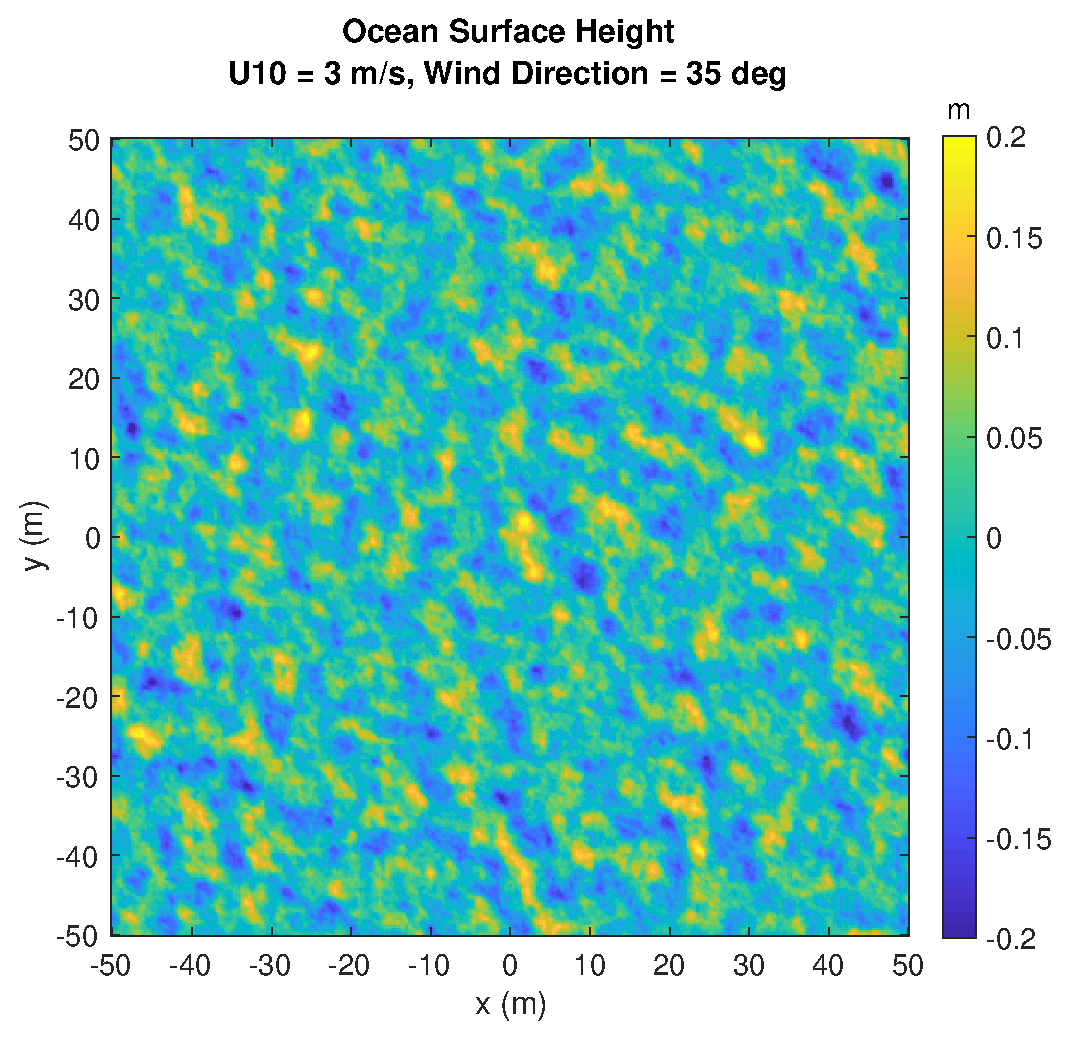
\includegraphics[width=3in]{RandomObjects/Figures/oceansurfaceheight} 
   \caption{Simulated wave heights at $t=0$ for $U_{10} = 3$ m/s, and $\theta_{\textrm{v}} = 35^o$.}
   \label{fig:3}
\end{figure}


The function \texttt{psdOcean} produces the 2D ocean wave PSD as a combination of the Pierson-Moskowitz 1D omnidirectional spectrum and a wind direction spreading function. It also returns the $k$-space components which are needed to evolve the surface.  The routine \texttt{evolveOcean} creates the surface at one instance in time, taking as inputs the ocean PSD and wavenumber components from \texttt{psdOcean} and one realization of $\gamma$.  Use the string switch \texttt{creamer2} to activate the nonlinear term. Numerically, the RMS wave height of the generated ocean surface does not always match the analytical value, therefore, consider renormalizing the surface RMS to the value given by \eqref{oceanrms}. 


{\scriptsize
\VerbatimInput{\code/RandomObjects/psdOcean.m}
}

{\scriptsize
\VerbatimInput{\code/RandomObjects/evolveOcean.m}
}

%\begin{figure}[htbp] 
%   \centering
%   \includegraphics[width=3.5in]{waveseries} 
%   \caption{Time series of wave heights.  Left to right, top to bottom, for $t = [0,1]$ seconds sampled at 0.125 seconds.  }
%   \label{fig:4}
%\end{figure}

\newpage

\section{Gaussian Random Particles}

In this section we give a procedure for creating and computing a spherical particle with Gaussian surface roughness. This is based on the formulation in \cite{muinonen1996light}. Specifically, the radius of the particle surface has log-normal statistics and the radii are correlated through a circular isotropic Gaussian angular correlation function. We have added 1) a derivation for the spherical harmonic expansion coefficients of the angular correlation function, which was not included in the paper, 2) computation using normalized Legendre polynomials, as well as 3) a stable way to carry out the computation in the small correlation limit.

%\subsubsection{Log-normal Radius}
\paragraph{Log-normal Radius}
From \cite{muinonen1996light}, the particle radius at spherical coordinate $(\theta,\phi)$ is described by the log-normal distribution
\eq{r(\theta,\phi) = \dfrac{a}{\sqrt{1 + \sigma^2}} \exp\left[s(\theta,\phi) \right]}

\noindent which has mean $a$, and variance $a^2\sigma^2$, where $s(\theta,\phi)$ is a zero-mean Gaussian random variable at each point $(\theta,\phi)$ with variance $\beta^2$.  The covariance of $s$ between two spherical points $(\theta_i,\phi_i)$, $(\theta_j,\phi_j)$ is given by 
\eq{\Sigma_{s,ij} = \beta^2 C_s(\gamma_{ij})}

\noindent where $\gamma_{ij}$ is the angular correlation between directions $i$ and $j$ and $C_s$ is the correlation function.  The covariances and distribution parameters are related as 
\ea{\Sigma_{r,ij} &=& a^2 \left[ \exp(\Sigma_{s,ij}) - 1 \right] \\
\sigma^2 C_r &=& \exp(\beta^2 C_s) - 1 \\
\sigma^2 &=& \exp(\beta^2) - 1}


%\subsubsection{Spherical Harmonic Expansion}
\paragraph{Spherical Harmonic Expansion}
The random variable, $s$, and angular correlation function are expressed in terms of real-valued spherical harmonics and associated Legendre polynomials, respectively, as
\eq{s(\theta,\phi) = \sum_{l=0}^{\infty} \sum_{m=0}^l P_l^m(\cos\theta)(a_{lm}\cos(m\phi) + b_{lm} \sin(m\phi)) \label{expansion} }
\eq{C_s(\gamma) = \sum_{l=0}^{\infty} c_l P_l(\cos\gamma) \label{correlationexp}}

\noindent where $a_{lm}$ and $b_{lm}$ are zero-mean Gaussian random variables with variance 
\eq{\beta^2_{lm} = (2- \delta_{m,0}) \dfrac{(l-m)!}{(l+m)!} \beta^2 c_l }

The correlation function is chosen as a spherical Gaussian of the form:
\ea{C_s(\gamma) &=& \exp\left( -\dfrac{2}{ l_c^2} \sin^2(\gamma/2) \right)  \label{correlation} \\ 
l_c &=& 2 \sin(\Gamma/2) }

\noindent where $l_c$ is the angular correlation (unitless) and $\Gamma$ is the correlation angle (radians). The function is circular such that the derivative at $\gamma=0$ and $\gamma=\pi$ is zero. The maximum correlation angle is $\Gamma = \pi$, for which the value at the maximum angle of separation, $\gamma = \pi$, is $\exp(-1/2) \approx 0.61$. Using \eqref{correlationexp}, \eqref{correlation} and orthogonality (derivation below) the expansion coefficients for the correlation function are 
\eq{c_l  = (2l+1) \exp\left( -\dfrac{1}{l_c^2}\right)  i_l\left( \dfrac{1}{l_c^2}\right)}

\noindent where $i_l(x)$ is the modified spherical Bessel function of the first kind. The number of required harmonics in the expansion increases as the correlation length decreases.  \cite{muinonen1996light} uses the following heuristic for 5 digits of precision:
\eq{L_{max} = \dfrac{275^o}{\Gamma} + 2.5}

\begin{figure}[h] 
   \centering
   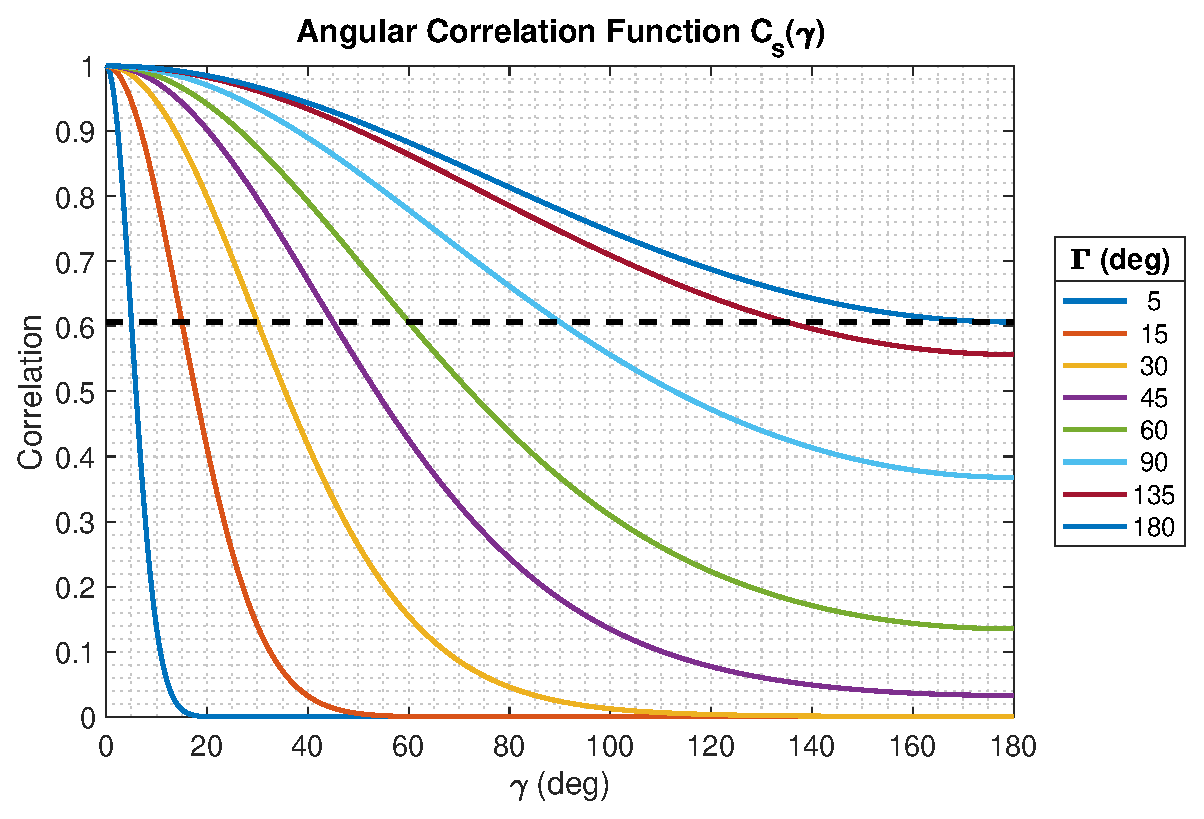
\includegraphics[width=3.5in]{RandomObjects/Figures/GaussianParticles/csgamma} 
   \caption{Angular correlation function, $C_s(\gamma)$.}
   \label{}
\end{figure}


%\subsubsection{Derivation of $c_l$}
\paragraph{Derivation of $c_l$}
A derivation for $c_l$ was not included in \cite{muinonen1996light}.  Applying orthogonality of the Legendre polynomials in \eqref{correlationexp}, the expansion coefficients of the correlation function are generally
\eq{c_l    = \dfrac{2l+1}{2}\int_0^{\pi} C_s(\gamma) P_l(\cos\gamma) \sin\gamma d \gamma }

%Applying orthogonality to \eqref{correlationexp}
%\eq{\int_0^{\pi} C_s(\gamma) P_n(\cos\gamma) \sin\gamma d \gamma  = \int_0^{\pi}\sum_{l=0}^{\infty} c_l P_l(\cos\gamma)P_n(\cos\gamma) \sin\gamma d \gamma}
%
%and using the relations
%\eq{x = \cos\gamma }
%\eq{\gamma = \arccos x }
%\eq{\int_{-1}^{1} P_n(x) P_m(x) dx = \dfrac{2}{2 n + 1} \delta_{mn}}

Using $\sin^2(\gamma/2) = (1 - \cos \gamma)/2$, the correlation function can be written
\eq{C_s(\gamma) = \exp\left( -\dfrac{1}{ l_c^2} (1 - \cos\gamma) \right) =  \exp\left( -\dfrac{1}{ l_c^2}\right)\exp\left(\dfrac{1}{ l_c^2} \cos\gamma \right)}

\noindent after which the integral becomes
\eq{c_l    = \dfrac{2l+1}{2} \exp\left( -\dfrac{1}{ l_c^2}\right)  \int_0^{\pi} \exp\left( \dfrac{1}{ l_c^2} \cos\gamma \right) P_l(\cos\gamma) \sin\gamma d\gamma \label{cltmp}}

From \cite{neves2006analytical, gouesbet1994rigorous}, this integral has the form
\eq{\int_0^{\pi} \exp\left[\pm i R \cos\theta\right] P_{l}^{\vert m \vert}(\cos\theta) \sin^{\vert m \vert + 1}\theta d\theta = 2 (\pm i)^{l+\vert m \vert} \dfrac{(l + \vert m \vert)!}{(l - \vert m \vert)!} \dfrac{j_l(R)}{R^{\vert m \vert}}}

%Using $m=0$ and identifying $- i R = 1/l_c^2$ it becomes
%\eq{\int_0^{\pi} \exp\left[\pm i R \cos\theta\right] P_{l}(\cos\theta) \sin\theta d\theta = 2 (\pm i)^{l} j_l(R) \label{simplifiedint}}

%Identifying
%\eq{ - i R = \dfrac{1}{l_c^2}}

Using $m=0$ and identifying $- i R = 1/l_c^2$, then \eqref{cltmp} reduces to
\eq{c_l  = \dfrac{2l+1}{2} \exp\left( -\dfrac{1}{ l_c^2}\right)  2 (-i)^{l} j_l\left( i  \dfrac{1}{l_c^2}\right)}

Using $(-i)^n = i^{-n}$, and the fact that $i_n(x) = i^{-n} j_n(i x)$, where $i_n(x)$ is the modified spherical Bessel function of the first kind,
\eq{i_n(x) = \sqrt{\dfrac{\pi}{2 x}} I_{n+1/2}(x)}

\noindent the expansion coefficients for the correlation function simplify to 
\eq{c_l  = (2l+1) \exp\left( -\dfrac{1}{ l_c^2}\right)  i_l\left(  \dfrac{1}{l_c^2}\right) \label{cl}}

\begin{figure}[H] 
   \centering
   \begin{tabular}{cccc}
 \subfigure{\includegraphics[width=2.1in]{RandomObjects/Figures/GaussianParticles/part7}}
 \subfigure{\includegraphics[width=2.1in]{RandomObjects/Figures/GaussianParticles/part8}}
 \subfigure{\includegraphics[width=2.1in]{RandomObjects/Figures/GaussianParticles/part9}}
 \\
  \subfigure{\includegraphics[width=2.1in]{RandomObjects/Figures/GaussianParticles/part4}}
 \subfigure{\includegraphics[width=2.1in]{RandomObjects/Figures/GaussianParticles/part5}}
 \subfigure{\includegraphics[width=2.1in]{RandomObjects/Figures/GaussianParticles/part6}}
  \\
 \subfigure{\includegraphics[width=2.1in]{RandomObjects/Figures/GaussianParticles/part1}}
 \subfigure{\includegraphics[width=2.1in]{RandomObjects/Figures/GaussianParticles/part2}}
 \subfigure{\includegraphics[width=2.1in]{RandomObjects/Figures/GaussianParticles/part3}}
% \\
% \subfigure{\includegraphics[width=2.1in]{RandomObjects/Figures/GaussianParticles/part1}}
% \subfigure{\includegraphics[width=2.1in]{RandomObjects/Figures/GaussianParticles/part2}}
% \subfigure{\includegraphics[width=2.1in]{RandomObjects/Figures/GaussianParticles/part3}}
% \subfigure{\includegraphics[width=2.1in]{RandomObjects/Figures/GaussianParticles/part4}}
\end{tabular}
\caption{Examples of Gaussian random particles with mean radius, $a=1$, for different log-normal RMS, $a\sigma$, and angular correlations, $\Gamma$.  Each correlation value requires a different number of total harmonics, however the spherical harmonics coefficients are computed from the same random seed (i.e., the random draws count up from the lowest harmonic), which ensures that the same features are observed across the different particles.}
\end{figure}

\clearpage
%\subsubsection{Fully Normalized Legendre Polynomials}
\paragraph{Fully Normalized Legendre Polynomials}
Equation \eqref{expansion} is best computed with the fully normalized Legendre polynomials, which avoid direct computation of the factorials. Defining $a_{lm}'$ and $b_{lm}'$ as draws from standard normal distribution with zero mean and unit variance, \eqref{expansion} can be written 
 \eq{s(\theta,\phi) = \sum_{l=0}^{\infty} \sum_{m=0}^l P_l^m(\cos\theta) \sqrt{(2- \delta_{m,0}) \dfrac{(l-m)!}{(l+m)!}  c_l} \beta (a_{lm}'\cos(m\phi) + b_{lm}' \sin(m\phi)) \label{stmp1}}

%\ea{a_{lm} &=& \beta_{lm} N(0,1) \\
%b_{lm} &=& \beta_{lm} N(0,1) }

The fully normalized associated Legendre polynomials are 
\eq{\widetilde{P}_l^m(x) = \sqrt{\dfrac{(l + 1/2)(l - m)!}{(l+m)!} } P_l^m(x) \label{fullynorm}}

Substituting \eqref{cl} into \eqref{stmp1} and using \eqref{fullynorm}, we get 
%\eq{s(\theta,\phi) = \sum_{l=0}^{\infty} \sum_{m=0}^l P_l^m(\cos\theta) \sqrt{(2- \delta_{m,0}) \dfrac{(l-m)!}{(l+m)!}  (2l+1) \exp\left( -\dfrac{1}{ l_c^2}\right)  i_l\left(  \dfrac{1}{l_c^2}\right)} \beta (a_{lm}'\cos(m\phi) + b_{lm}' \sin(m\phi))}

\eq{s(\theta,\phi) = \beta \sum_{l=0}^{\infty} \sum_{m=0}^l c_{lm}'  \widetilde{P}_l^m(\cos\theta)  (a_{lm}'\cos(m\phi) + b_{lm}' \sin(m\phi))}

\noindent where 
\eq{c_{lm}' =   \sqrt{2 (2- \delta_{m,0})  \exp\left( -\dfrac{1}{ l_c^2}\right)  i_l\left(  \dfrac{1}{l_c^2}\right)}}


%\subsubsection{Small Correlation Limit}
\paragraph{Small Correlation Limit}
When the correlation angle is small, e.g., $\Gamma < 3^o$, the following computation is problematic
\eq{A_l(l_c) = \exp\left( -\dfrac{1}{ l_c^2}\right)  i_l\left( \dfrac{1}{l_c^2}\right) \label{allc}}

\noindent because the exponent goes to zero and the Bessel function becomes large.  The solution is to use the log transform as well as recursion over the series expansion of the Bessel function. From \cite[Eq.~10.53.3]{NIST:DLMF}, the series expansion of the modified Bessel function is 
\eq{i_l(z) = z^l \sum_{k=0}^{\infty} \dfrac{(1/2 z^2)^k}{k! (2l + 2k + 1)!!}} 

Setting $z = 1/l_c^2$ and pulling all terms into the sum \eqref{allc} can be written  
\eq{A_l(z) = \sum_{k=0}^{\infty} e^{-z} z^l  \dfrac{(1/2 z^2)^k}{k! (2l + 2k + 1)!!} = \sum_{k=0}^{\infty} a_{l,k} } 

Using the log transform, the terms of the sum are expressed as $a_{l,k} = e^{\ln a_{l,k}}$. Writing out the logarithm
\eq{\ln a_{l,k} = -z + l \ln z + k(-\ln 2 + 2 \ln z) - \ln k! - \ln (2l + 2k + 1)!! \label{logtemp}}
%\eq{A_l(z) = \sum_{k=0}^{\infty} e^{\ln a_{l,k}} }
%\eq{A_l(z) = \sum_{k=0}^{\infty} e^{\ln a_{l,k}} }
The double factorial for odd integers is $n!! = \prod_{k=1}^{(n+1)/2} (2k - 1)$. Using this in \eqref{logtemp} and converting the products to sums
\eq{\ln a_{l,k} = -z + l \ln z + k(-\ln 2 + 2 \ln z) - \sum_{n=1}^k \ln n - \sum_{n=1}^{l+k+1} \ln (2n - 1)}
%or
%\ea{(2l + 2k + 1 )!! %&=& \prod_{n=1}^{(2l + 2k + 1+1)/2} (2n - 1) \\
%&=& \prod_{n=1}^{l+k+1} (2n - 1)}


To avoid recomputing the sums for new $l$ and $k$, fast recursion relations are derived by writing out $l+1$ or $k+1$ and separating $\ln a_{l,k}$: 
\ea{\ln a_{l+1,k} &=& \ln a_{l,k} + \ln z  - \ln (2(l+k) + 3) \label{lrecur} \\
\ln a_{l,k+1} &=&   \ln a_{l,k}  -\ln 2 + 2 \ln z - \ln (k+1) - \ln(2(l+k) + 3) \label{krecur}}

%\ea{\ln a_{l+1,k} &=&  -z + (l+1) \ln z + k(-\ln 2 + 2 \ln z) - \sum_{n=1}^k \ln n - \sum_{n=1}^{l+1+k+1} \ln (2n - 1)  \\
%\ &=& -z + l \ln z + \ln z + k(-\ln 2 + 2 \ln z) - \sum_{n=1}^k \ln n - \sum_{n=1}^{l+1+k} \ln (2n - 1)  - \ln (2(l+1+k+1) - 1)  \\
%\ &=& \ln a_{l,k} + \ln z  - \ln (2(l+k) + 3) \label{lrecur}}

%To derive a recursion relation in $k$, write out $k+1$, and separate $\ln a_{l,k}$ 

%\ea{\ln a_{l,k+1} &=&  -z + l \ln z + (k+1) (-\ln 2 + 2 \ln z) - \sum_{n=1}^{k+1} \ln n - %\sum_{n=1}^{l+k+1+1} \ln (2n - 1) \\
%\ &=& -z + l \ln z + k(-\ln 2 + 2 \ln z) +  (-\ln 2 + 2 \ln z)  - \sum_{n=1}^k \ln n -  \ln (k+1) - \sum_{n=1}^{l+k+1} \ln (2n - 1) - \ln (2(l + k+2) - 1)  \\
%\ &=& \ln a_{l,k}  -\ln 2 + 2 \ln z - \ln (k+1) - \ln(2(l+k) + 3) \label{krecur}}

The procedure is to compute $a_{l,0}$ (up to a given $L$) using \eqref{lrecur}, then recurse over $k$ using \eqref{krecur} until convergence. The convergence will be different for each $l$.  Using $k=0$ in \eqref{lrecur}, $a_{l,0}$ are computed with: 
\eq{\ln a_{l+1,0}=  \ln a_{l,0} + \ln z  - \ln (2l + 3) }

\noindent where $\ln a_{0,0} = -z $. 

\paragraph{Routine}
The routine \texttt{gaussianRandomParticle} takes as input the coordinates $(\theta,\phi)$, mean radius of the particle, log-normal surface RMS, and correlation angle, and returns the radius of the surface at each spherical point computed with the methods above. The maximum degree $L$ is optional and defaults to the heuristic. It computes the harmonic sum directly to allow input of any sampling of $(\theta,\phi)$, but this is inefficient for a large number of points and small correlation angles (because $L$ is large), even though the computation is correct. If the spherical angles can be sampled at the points of quadrature, the particle surface could be computed using a fast spherical transform, which is mentioned here for future development. Alternatively, a version of this in which the Legendre polynomials are computed on the fly with inline recursion could be developed to save memory.

{\footnotesize
\VerbatimInput{\code/RandomObjects/gaussianRandomParticle.m}
}

\clearpage

\section{Ionosphere Irregularity}
\paragraph{Background} Earth's ionosphere is a complex plasma medium that exists at altitudes between 100 km and 600 km and affects the propagation of radio, radar, and GPS signals. The influence of the ionosphere on these signals increases as the radio frequency decreases. It starts to affect radar around L-band (1-2 GHz) and UHF-band (300 MHz - 1 GHz), becomes a significant dispersive medium in the VHF band (30-300 MHz), and is completely reflecting in the HF band below the plasma frequency (around 10 MHz). The strength of the ionosphere is highly dependent on the time of day and latitude. The ionosphere is always changing, but a given 3D spatial distribution of electron density can usually be considered constant over a short time duration, for example, of a synthetic aperture radar acquisition from an orbiting spacecraft.  

The simplest parameters that quantify the ionosphere are 1) electron density, $N_e$, which is a function of altitude and given in terms of number of electrons per unit volume (el/m$^3$), 2) the total electron content (TEC) which is the column-integrated electron density up to a given altitude, given in terms of number of elections per unit area (el/m$^2$), and 3) irregularities that are random fluctuations in the spatial distribution of the plasma density. The TEC is given by 
\eq{TEC(h) = \int_{0}^{h} N_e(z) dz}

\noindent where $N_e(z)$ is the electron density as a function altitude, and $h$ is the altitude up to which we wish to evaluate the TEC. TEC is often the only parameter needed to assess the two-way effects of the ionosphere on the radar signal such as dispersion, Faraday rotation, and absorption loss. Irregularities contribute to scintillation, which are fluctuations of the phase and amplitude of the radar echo about a mean response. Scintillation creates small phase variations across a synthetic aperture, and these phase variations lead to decoherence and a drop in coherent gain when creating images. While strong ionospheric dispersion at VHF frequencies is almost completely correctable, scintillation is often uncorrectable, because there is no way to predict what the irregularities will be at a given time or place. Finally, the study of Earth's ionosphere spans many decades, and more information on these topics can be found in the literature.

\paragraph{Formulation} We give a routine for creating a 1D profile of ionospheric irregularities that is suitable for radar analysis. This is based on the 2-parameter PSD model in \cite{liu2003ionospheric,ishimaru1999ionospheric}, from which 1D profiles can be created using the methods from Section \ref{sec:1drandom}. The 2-parameter model effectively creates different regimes of roughness that define the underlying structure of the irregularity. These are controlled through two log-slope regions in the PSD. The log-slope values come from empirical observations, while the mean and relative variation are set by user-defined scale factors. The signal can be scaled to either electron density, assuming a uniform column, or to the TEC itself. The scale factors in this model are not very informative, however, computing actual TEC and irregularity amplitude is quite complicated. A more informative model is given, for example, in \cite{rogers2013impacts}, which provides a PSD of radar phase scintillation using scale factors from up-to-date global ionospheric models. Still, the use of user-defined scale factors can suffice for first-order analysis.

From \cite{liu2003ionospheric,ishimaru1999ionospheric}, the 2-parameter PSD for the electron density irregularity is given for 3D $k$-space as 
\eq{\Phi(k) = \begin{cases}
\dfrac{A}{(k^2 + k_o^2)^{v_1}} & k \le k_b \\
\\
\dfrac{A(k_o^2 + k_b^2)^{v_2-v_1}}{(k^2 + k_o^2)^{v_2}} & k > k_b \\
\end{cases}}

\noindent where $k$ is the spatial wavenumber, $k_o = 2\pi/L_o$ is the outerscale wavenumber at length scale $L_o$, $k_b = 2\pi/L_b$ is the break wavenumber at length scale $L_b$, $v_1$ and $v_2$ are log-slope parameters, and $A$ is a scale factor. The values for the parameters are empirical and cited in \cite{ishimaru1999ionospheric} as: $L_o \approx 10$ km, $L_b \approx 500$ m, $2v_1\approx$  3-3.5, and $2v_2\approx$  5-5.5.  

The 1D PSD, $V(k)$, is related to the 3D PSD as \cite{ishimaru1978wave}
\eq{\Phi(k) = -\dfrac{1}{2\pi k} \dd{V(k)}{k}}

which leads to the 1D PSD, \cite{liu2003ionospheric}, 
\eq{V(k_x) = \begin{cases}
\dfrac{\pi A}{v_1 - 1}\dfrac{1}{(k_x^2 + k_o^2)^{v_1-1}} - \dfrac{\pi A}{(k_b^2 + k_o^2)^{v_1-1}}\left(\dfrac{1}{v_1-1} - \dfrac{1}{v_2-1} \right) & k_x \le k_b \\
\\
\dfrac{\pi A(k_o^2 + k_b^2)^{v_2-v_1}}{v_2-1}\dfrac{1}{(k_x^2 + k_o^2)^{v_2-1}} & k_x > k_b \\
\end{cases} \label{scintpsd}}

\noindent where $k_x$ is now a 1D wavenumber. The key feature of this PSD are two regimes of log-slope power. 

The 1D profile of electron density, $N_e(x)$, is realized by multiplying each frequency of the PSD with a draw from a complex standard normal distribution and then taking the inverse Fourier transform. The amplitude, $A$, has so far been arbitrary, but it is there to adjust the scale of the signal. Let $n_e(x)$ be a zero mean profile generated by \eqref{scintpsd} which is normalized by its RMS. This signal can then be rescaled as
\eq{N_e(x) =  \overline{N}_e \left( \tilde{\sigma} n_e(x) + 1\right) \label{iononorm}}

\noindent where $\overline{N}_e$ is the average electron density and $\tilde{\sigma}$ is the relative RMS variation given as a fraction, or percentage, of the mean. This assumes that the ionospheric column has uniform electron density. Alternatively, \eqref{iononorm} can be used for TEC if $\overline{N}_e$ and $\tilde{\sigma}$ are replaced by the average TEC and percentage RMS variation in TEC, respectively. %Note, it is unclear from \cite{liu2003ionospheric} if the relative variation, $\tilde{\sigma}$, is supposed to be peak to peak, the RMS, or 2 times the RMS. We define $\tilde{\sigma}$ as the relative RMS of the signal after subtracting the mean. 


\begin{figure}[H] 
   \centering
   \subfigure{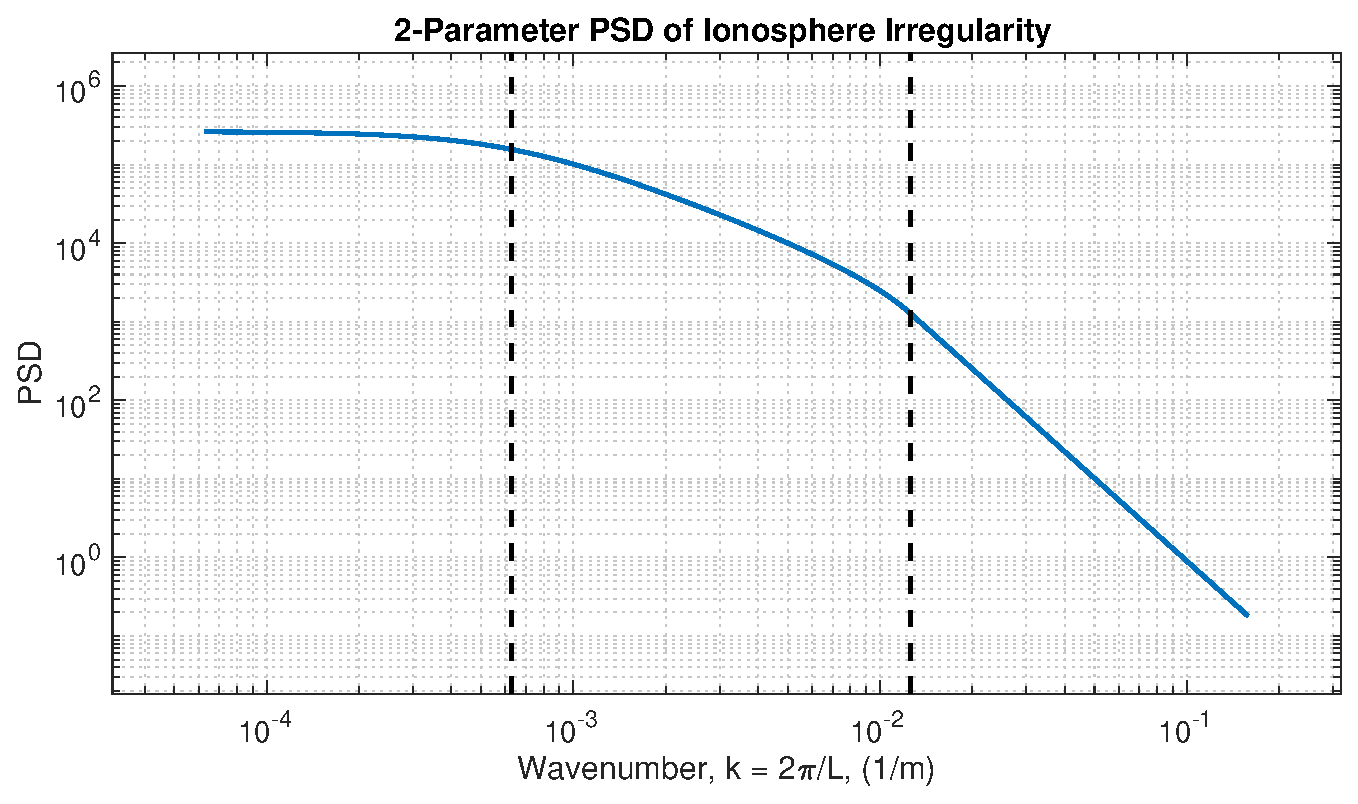
\includegraphics[width=3in]{RandomObjects/Figures/ionoPSD1} }
      \subfigure{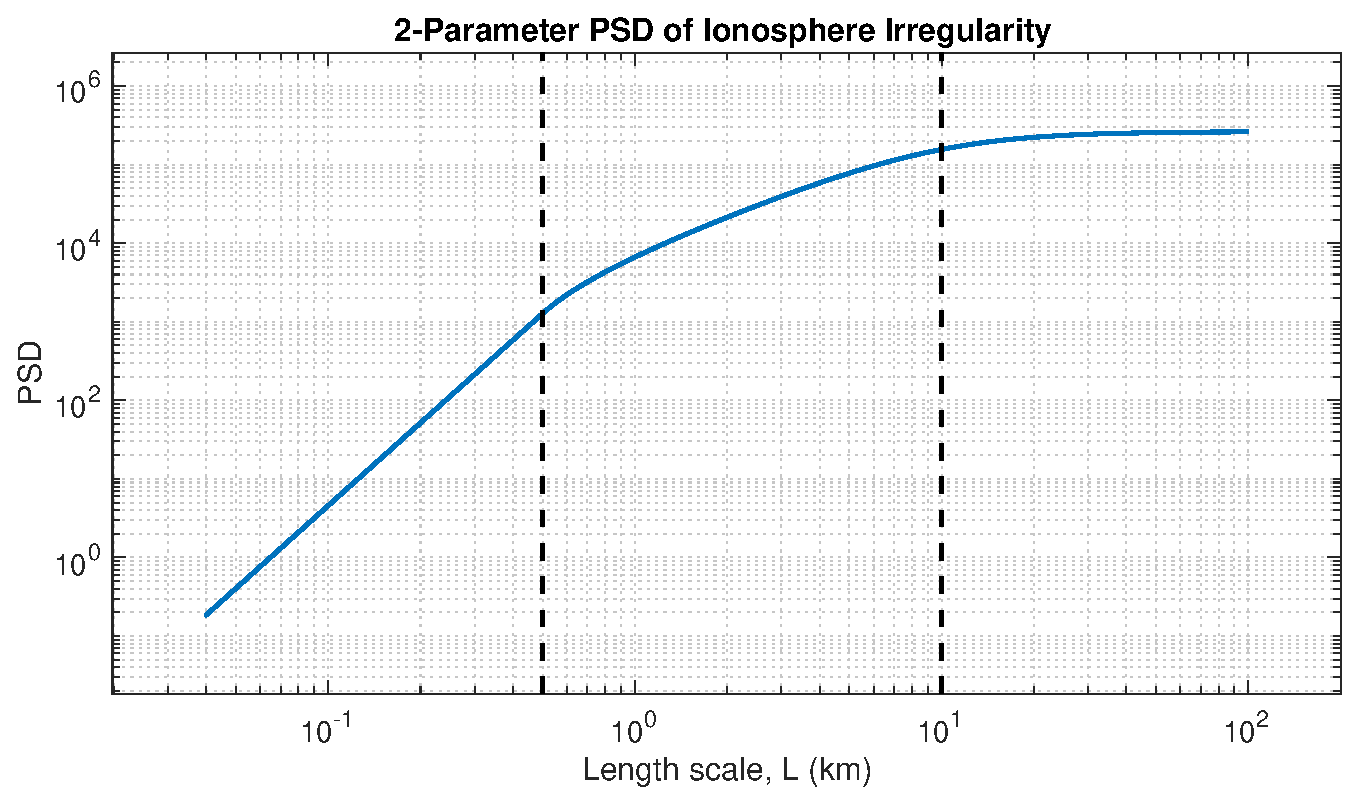
\includegraphics[width=3in]{RandomObjects/Figures/ionoPSD2} }        
   \caption{PSD of ionosphere irregularity with respect to wavenumber (left) and length scale (right) for the default parameters: $L_o = 10$ km, $L_b = 500$ m, $2v_1=$ 3.5, and $2v_2=$ 5.5.  Dashed lines are the outerscale and breakscale. The end points of the curves correspond to the wavenumber or length scale of the total profile length or the sampling step. }
\end{figure}

\begin{figure}[H] 
   \centering
 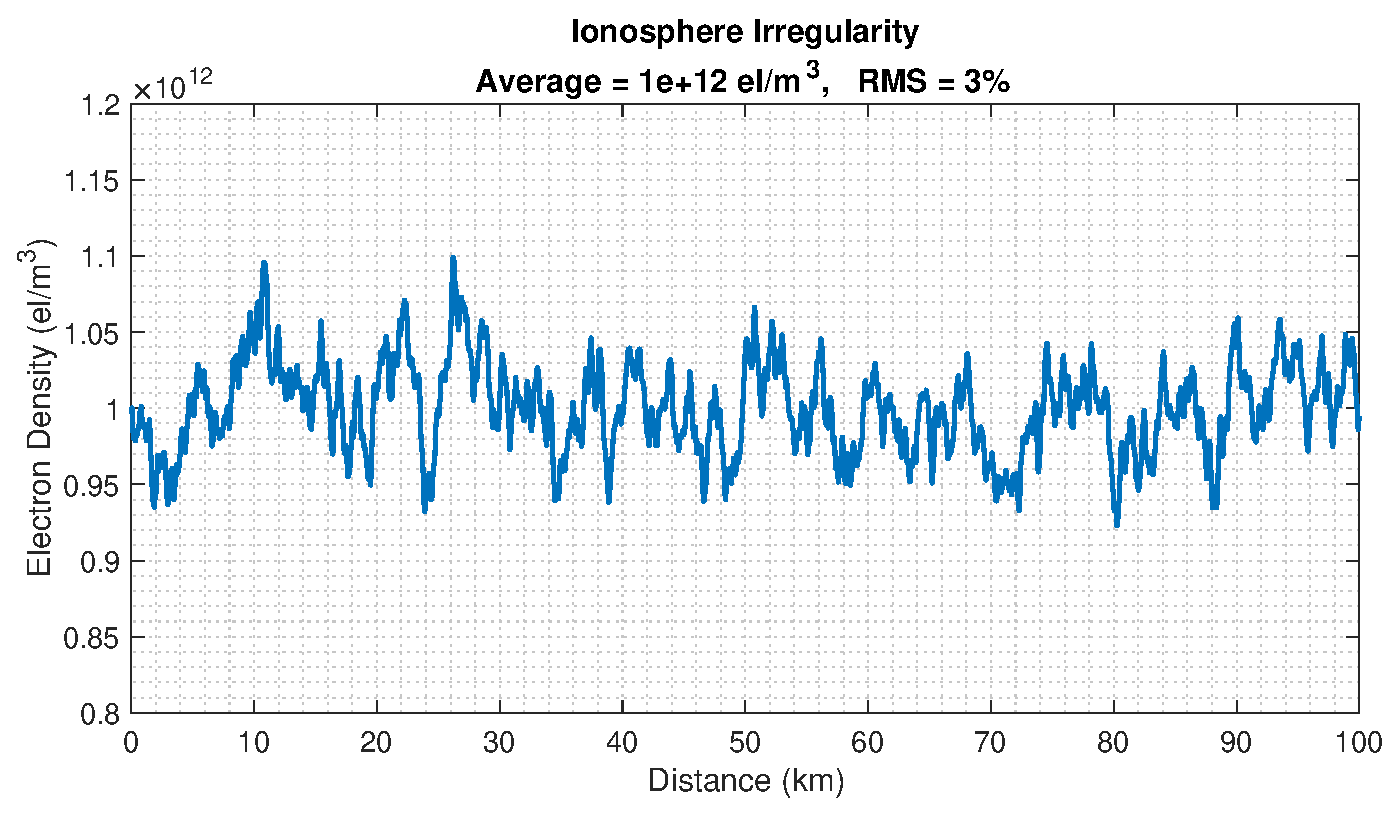
\includegraphics[width=4in]{RandomObjects/Figures/ionoProfile} 
   \caption{Profile of ionosphere irregularity for the default parameters: $L_o = 10$ km, $L_b = 500$ m, $2v_1=$3.5, and $2v_2=$5.5. Numerically, the correlation length was found to be about 1 km. }
\end{figure}

\paragraph{Routine} The routine \texttt{ionosphere1} produces a 1D profile of ionosphere irregularity based on the 2-parameter PSD above. It takes as input the number of sample points, profile length, average value, and relative RMS variation in percentage of the mean. The scale factors can be electron density or TEC. It uses the same generating procedure as \texttt{rough1} in Section \ref{sec:1drandom}. Default model parameters are: $L_o = 10$ km, $L_b = 500$ m, $2v_1=$3.5, and $2v_2=$5.5. Different values can be optionally included as input arguments, in the same order, where an input of \texttt{'[]'} will use the default value. The routine can output the PSD, wavenumber, and model parameters for plotting.


{\footnotesize
\VerbatimInput{\code/RandomObjects/ionosphere1.m}
}


%\section{Fractals}
%
%Fractals are not computed with PSDs, so we treat them separately.  From Tsang, one type of 1D fractal is given by the Weierstrass-Mandelbrot function.  
%
%\[ f(x) = h C \sum_{n=0}^{N-1} b^{(s-2)n} \sin\left(k_L b^n x + \Phi_n\right) \]
%
%\noindent where
%
%\begin{eqnarray}
%h &=& \textrm{RMS height} \nonumber \\
%N &=& \textrm{number of modes} \nonumber \\
%s &=& \text{fractal dimension} \quad (1 \le s < 2) \nonumber \\
%C &=& \sqrt{\dfrac{2\left(1-b^{2(s-2)}\right)}{1- b^{2(s-2)N} }} = \textrm{normalization constant} \nonumber \\
%\Phi_n &=& \textrm{phase term drawn for each mode from a uniform distribution between 0 and $2\pi$}\nonumber 
%\end{eqnarray}
%
%The signal is band limited between wave numbers $k_L$ and $k_U$ through the relations
%
%\begin{eqnarray}
%k_U &=& k_L b^{N-1} \\
%b &=& \left(\dfrac{k_U}{k_L} \right)^{\frac{1}{N-1}} 
%\end{eqnarray}
%
%We can convert the band limits into the more intuitive length scales
%
%\begin{eqnarray}
%l_U  &=& \dfrac{2\pi}{k_L} \\
%l_L &=& \dfrac{2\pi}{k_U} 
%\end{eqnarray}
%
%\noindent where $l_U$ and $l_L$ are the longest and shortest length scales, respectively, of the surface roughness.  Because we ultimately sample this function, our smallest length scale must satisfy Nyquist.  Let $L_x$ be the extent of the surface and $N_x$ be the number of samples, then the smallest allowable length scale is 
%
%\[ l_L >  l_{\textrm{min}} = \dfrac{N_x-1}{\pi L_x} \]
%
%The routine \texttt{fractal1} implements this function.  $l_L$ is checked and set to $1.05 l_{min}$ if Nyquist is not satisfied in order to prevent aliasing.  This way you can choose the sample rate as it relates to the problem at hand.  As long as $l_U$ is not too large (and $k_L$ close to zero), the signal is mostly zero mean.  Increasing the modes increases the density of frequency components in the band, but be generous in order for the fractal shape to be realized (e.g., $N > $ 100).  One last note, because this fractal is just a sum of sinusoids, it has continuous derivatives.  The first derivative is an optional output.
%
%
%{\footnotesize
%\VerbatimInput{\code/RandomObjects/fractal1.m}
%}
% 
% \begin{figure}[h] 
%   \centering
%   \includegraphics[width=5in]{RandomObjects/fractal1} 
%   \caption{1D fractal surface and spectrum. $N_x =$ 500 samples, $L_x =$ 200 m, RMS = 1 m, $l_L =$ 1 m, $l_U =$ 20 m, $s =$ 1.5, $N =$ 100.}
%\end{figure}


